\documentclass[12pt,a4paper]{article}
%**************************************************************************************************
% PACKAGES
%**************************************************************************************************
\usepackage{amsmath, amsthm, amsfonts, amssymb}
\usepackage{graphicx,color}
\usepackage{bm}	
\usepackage{hyperref}
\usepackage{a4wide}
\usepackage{caption}
\usepackage{subcaption}
\usepackage[framemethod=tikz]{mdframed}
\usetikzlibrary{shadows}
\newmdenv[shadow=true,shadowcolor=black,rightmargin=-8pt]{shadedbox}
\newtheorem{theorem}{Theorem}
\newtheorem{definition}[theorem]{Definition}
\newtheorem{corollary}[theorem]{Corollary}
\newtheorem{example}[theorem]{Example}
\newtheorem{lemma}[theorem]{Lemma}
\newtheorem{algorithm}[theorem]{Algorithm}
\usepackage{setspace}
\newenvironment{bigexample}{\begin{shadedbox}\begin{example}\normalfont}{\end{example}\end{shadedbox}}
%\singlespacing
%\onehalfspacing
%\doublespacing
%\setstretch{1.1}
%**************************************************************************************************
% DEFAULT SETTINGS
%**************************************************************************************************
\parskip= 1 ex
\columnseprule = 0.1pt
\footskip = 30 true pt
\hoffset = -0.1 true in
\voffset = -0.1 true in
\abovedisplayskip 1 true pt
\abovedisplayshortskip 1 true pt

%**************************************************************************************************
% DOCUMENT DETAILS
%**************************************************************************************************

\title{An Introduction to Differential Cryptanalysis of Block Ciphers}
\author{Steven Rybicki (RYBSTE001)}
\date{}
%**************************************************************************************************
% MAIN DOCUMENT 
%**************************************************************************************************
\newcommand{\differ}[1] {\overset{#1}{\rightarrow}}
\newcommand{\bin}[1] {0b#1}
\newcommand{\binp}[1] {\,\text{0b#1}\,}
\newcommand{\hex}[1] {0x#1}
\newcommand{\hexp}[1] {\,\text{0x#1}\,}
\begin{document}
\maketitle
\begin{abstract}
Block ciphers, ciphers that take blocks of input, are used in cryptography to
encrypt data and build other cryptographic schemes. This is only possible if
block ciphers have the confidentiality property: any text encrypted under a
secret key with that block cipher is not able to be decrypted without that key.
In this project we discuss differential cryptanalysis and how this can be used
to break the confidentiality of certain substitution-permutation network based
block ciphers. We start by outlining the basic results in probability and
cryptanalysis of substitution-permutation networks required to understand the
attack. We then go through the details of how to attack a cipher using
differential cryptanalysis, building the intuition required to understand how
this attack works and then applying this to a toy cipher. 
\end{abstract}
\newpage
\tableofcontents
\listoffigures
\listoftables
\newpage
%*********************************************************************************************************
\section{Preface}
%*********************************************************************************************************
\textit{Cryptanalysis} is the study of recovering information from ciphers
without knowing the secret key. \textit{Differential cryptanalysis} tries to
recover secret information from ciphers by looking at how the ``differences" in
pairs of inputs can affect the differences of the outputs. This field, while
first publicly disclosed by Biham and Shamir \cite{biham1991differential}, was
identified earlier and kept secret by the designers of DES (Data Encryption
Standard) as it was regarded as powerful enough of a weapon against ciphers to
be a national secret. Since then it has been used to great effect against a
number of ciphers.

While you can perform differential cryptanalysis on various kinds of ciphers,
in this project we are going to focus on applying it to block ciphers,
specifically iterated block ciphers designed as a substitution-permutation
network like Unsub A (see Appendix \ref{sec:UnsubA}). These terms are defined
later in the project.

In order to understand these attacks fully, one needs some background in
discrete probability and cryptanalysis. For those readers who have not have
been exposed to these concepts, we have provided a primer to get you up to
speed in Sections \ref{sec:probability} and \ref{sec:intro}. If you are familiar
with basic cryptanalysis concepts and discrete probability, or are not
interested in the theoretical basis for the attacks, simply skim over these
sections and start reading in earnest starting with Section \ref{sec:analysis}. 

In each section relating to the differential cryptanalysis and attack, we will
first try to develop the theoretical basis that can applied to all block
ciphers based on a substitution-permutation network. Where relevant we will
also give concrete examples of that attack or analysis as performed on Unsub A.
This is to ensure the reader has an understanding of why the analysis or attack
is relevant and valid as well as an example to ground this understanding. 

We are going to be basing our approach on the The Block Cipher Companion
\cite{BlockCipherCompanion}. All other sources will be cited when mentioned.

\newpage

\section{Discrete Probability Theory}
\label{sec:probability}
\subsection{Introduction}
We all have an intuitive sense of probability which we can use to predict the
likelihood of events: we know that winning the lottery is unlikely and that a
fair coin when flipped should come up heads as often as it comes up tails. In
each of these, we have an event (winning the lottery, a coin coming up heads)
and an associated probability (a small one and $\frac{1}{2}$). In this section,
we are going to take our intuitive understanding of probability and formalize
it.

Since this project is not a text on probability, we will give only a brief
introduction. If you want a more comprehensive treatment, see any good
mathematical text on discrete probability theory such as \textit{Grinstead and
Snell's Introduction to Probability} \cite{amsbook}. This text is available for
free under the GNU Free Document Licence \footnote{At the time of writing, a
copy is available at the following link:
\url{http://www.dartmouth.edu/~chance/teaching_aids/books_articles/probability_book/book.html}}.

Let us first look at what it means to say that ``An event $X$ will occur with
Probability $Y$". 

\begin{definition}
We call any procedure that a) we can repeat and b) has a set of well defined
outcomes an \textbf{experiment}. For any experiment, let the \textbf{sample
space} denote the all outcomes of this experiment. We will usually represent the
sample space by $\Omega$. If $X$ is a subset of $\Omega$, we call $X$ an
\textbf{event}.
\end{definition}

Let us take two every day events, flipping a fair coin and rolling a die, and
represent them using the concepts we introduced above.
\begin{example}
\label{exm:coin_events}
In the experiment of ``flipping a fair coin", the sample space would be the coin
coming up heads or tails\footnote{This holds if we ignore a coin landing on its side which
in this case we will.}. If we represent the result of a coin coming up
heads by $H$ and similarly represent the result of a coin landing on tails by
$T$, we have that for this experiment $\Omega = \{H,T\}$. Here, our events
are $\{H\}$,$\{T\}$ (the coin coming up heads or tails respectively),
$\emptyset$ (the coin comes up neither heads or tails) or $\Omega$ (the coin
comes up heads or tails).
\end{example}

Note that even though $\emptyset$ will never occur,
it is still a valid event as $\emptyset \subset \Omega$ for any sample space
$\Omega$.

\begin{example}
If we looked at the experiment of rolling a traditional six sided die and
examining its displayed value, we would have $\Omega = {1,2,3,4,5,6}$ with the
event $\{2,4,6\}$ corresponding to rolling an even number.
\end{example}

Now, with both of the above examples, each outcome occurs with equal
likelihood.  Rolling a 6 on a die is as likely as rolling a 1; flipping a fair
coin and getting heads is as likely as getting tails. However, not all elements
in a sample space occur with equal likelihood as our example below shows.
\begin{example}
\label{exm:picking}
Let us examine the experiment of you and a friend each picking an integer from
one to $10^{10}$ at random and seeing if they were equal. We would have 
\[\Omega =
\{\mbox{Numbers are equal},\mbox{Numbers are not equal}\}\]
In this sample
space, the event ``$\{\mbox{Numbers are not equal}\}$" is more likely to occur
than the event $\{\mbox{Numbers are equal}\}$.
\end{example}

For the dice and fair coins, we say that there is a \textit{uniform probability
distribution} - all individual outcomes occur with equal likelihood. However,
this is not always the case. So before we can define what a probability is, we
need to look at \textit{probability distributions}.

\begin{definition}[Probability Distribution]
A \textbf{probability distribution} for an experiment with sample space $\Omega$ is a
function $m:\Omega \rightarrow [0,1]$ such that
\[\sum_{x \in \Omega} m(x) = 1 \].

If $(\forall x \in \Omega)\; m(x) = \frac{1}{|\Omega|}$, then $m$ is said to be a
\textbf{uniform probability distribution}.
\end{definition}

With this in mind, we can define the concept of a probability.

\begin{definition}[Probability]
Given an experiment with sample space $\Omega$ and probability distribution $m$
over $\Omega$, the \textbf{probability} of an event $X$ is defined as a
function $Pr: 2^\Omega \rightarrow [0,1]$ where $2^\Omega$ is the \textbf{powerset}
of $\Omega$ (set of all subsets of $\Omega$) and
\[Pr[X] = \sum_{x \in X} m(x) \]
\end{definition}
Here, the powerset of our sample space $\Omega$ is simply the set of all
events. So in the case of Example \ref{exm:coin_events}, we have that
\[2^\Omega = \{\emptyset,\{H\},\{T\},\Omega\}\] The powerset of $X$ is also
sometimes represented as $P(X)$, but we prefer the $2^X$ notation as the number
of elements in the powerset of a finite set is $X$ is $2^|X|$. 

Loosely, the probability of an event $A$ corresponds to the likelihood
that $A$ occurs in our experiment where as our probability distribution
corresponds to the likelihood that a singleton from $\Omega$ occurs. 

Note that for a given probability distribution, the probability for an event is
fixed. Therefore if we have a case where we want to change the probability
associated with an event, we must change our probability distribution. This is
illustrated in the example below.

\begin{example} Let us consider flipping a fair coin versus flipping a biased
coin (a coin which lands on one side more often than another). Both have the
same sample space $\Omega=\{H,T\}$ but the probability of the coin landing
heads for each will be different. We represent this by giving them different
probability distributions. For the fair coin, we will have a uniform
distribution. For the biased coin, we would have $m(H) = p, m(T) = 1-p$ for
some $p \in [0,1]$.  \end{example}

There is an alternate way to introduce the concept of a probability which
involves using \textit{Kolmogorov's Axioms}. We are going to list these as
a theorem and prove them using the concept of probability defined
above. Note that as we go on, we will stop explicitly mentioning we are talking
about experiments and simply refer to their sample spaces, with the experiment
being made obvious by the context.
\begin{theorem}[Kolmogorov]
\label{thm:kol}
Given a sample space $\Omega$ for an experiment with a probability distribution
$m$ over $\Omega$ and events $A,B \subseteq \Omega$, we have that 
\begin{enumerate}
    \item $0 \leq Pr[A] \leq 1$
    \item $Pr[\Omega] = 1, Pr[\emptyset] = 0$
    \item If  $A \cap B = \emptyset$ then $Pr[A \cup B] = Pr[A] + Pr[B]$
\end{enumerate}
\end{theorem}

As this is a project on differential cryptography rather than probability, only
the sketches for the proofs are provided below.

\begin{proof}
We prove each of these separately.
\begin{enumerate}
\item Note that $Pr[X] = \sum_{x \in X} m(x)$. Since $m$ has a codomain of
$[0,1]$, for any $x \in \Omega, m(x) \geq 0$ which means that $\sum_{x \in X}
m(x) \geq 0$. For the other inequality, we note that
\[\sum_{x \in X} m(x) \leq \sum_{x \in X} m(x) + \sum_{x \in (\Omega - X)} m(x)
= \sum_{x \in \Omega} m(x) = 1\]

\item $Pr[\Omega] = \sum_{x \in \Omega} m(x) = 1$ and $Pr[\emptyset]
= \sum_{x \in \emptyset} m(x) = 0$ as there are no elements in the empty set. 

\item We will prove this for finite $\Omega$. Let us set $A = \{a_0, \ldots,
a_n\}$ and $B = \{b_0, \ldots, b_m\}$. Then we have that

\[Pr[A \cup B] = \sum_{x \in A \cup B} m(x) = m(a_0) + \ldots + m(a_n) + m(b_0)
+ \ldots + m(b_m) = \sum_{x \in A} m(x) + \sum_{x \in B} m(x)\] as their
intersections are empty. This gives $Pr[A \cup B] = Pr[A] + Pr[B]$.
\end{enumerate}
\end{proof}
\subsection{Random Variables}

In the previous section, we developed a language which we can use to describe
the probability of a specific event happening according to a probability
distribution over a sample space. However, we would like a more flexible way to
specify events like events that occur randomly. 

For example, consider the experiment of taking a card out of a deck. How would
you express the event ``Picked a red card"? We would simply create a set which
contain all the red cards. However, this approach becomes a bit less elegant
when we look at events like ``Picked a number card with value $i$" for some $i$
in $\{1,2,\ldots,9,10\}$. It is possible to do so with the concepts developed above, but
we would prefer a much more elegant way. To do this, we use \textit{Random
Variables}.

\begin{definition}[Random Varaibles]
For a sample space $\Omega$, a \textbf{random variable} is a function $r:\Omega
\rightarrow V$ where $V$ is a non-empty set.

For $v \in V$ we define the probability of the random variable $r$
taking the value $v$ over $\Omega$ to be $Pr[r=v] = Pr[r^{-1}(v)].$ 

If $V=\Omega$ and $r$ is $Id_\Omega$, i.e. the identity function on $\Omega$,
then $r$ is said to be the \textbf{uniform random variable} over $\Omega$.
\end{definition}
\begin{example}
Let us take the card experiment from above. To describe the event of picking a
red card, we would define a random variable $r$ to go to the set $\{1,0\}$ with $r$
being defined as sending all red cards to $1$ and all black cards to $0$. Then,
we can define the probability desired as $Pr[r=1]$. Similarly, if we wanted to define the
event ``Picked a number card with value 2", we would set $V =
\{0,2,\ldots,9,10\}$ with $r$ sending all number cards to their values and all
face cards (Ace, King, Queen, Jack) to 0. Then the probability for the event
would be \[Pr[r=2] = Pr[r^{-1}(2)] = Pr[\{2 \mbox{ of clubs} , 2 \mbox{ of
spades}, 2 \mbox{ of hearts}, 2 \mbox{ of diamonds}\}] = \frac{1}{13}\] as the
probability distribution for picking cards is uniform.
\end{example}

\subsection{Conditional Probability}

We now have a flexible way to describe probability distributions, but still no
elegant way to describe a sequence of events. For example, we might want to
know what the probability is that we draw an ace from a pack of cards given
that in the previous three draws we drew all aces. In order to do this, we
need to define what it means for something to follow conditionally from
something else. We also need some way of calculating this probability.

\begin{definition}[Conditional Probability]
Let $A$ and $B$ be events in $\Omega$. Then we represent the probability of $A$
occurring after $B$ is known to have occurred as 
\[Pr[A|B] = \frac{Pr[A \cap B]}{Pr[B]}\].

This is known as \textbf{conditional probability}.
\end{definition}

To give some intuition for this definition, let us reason about the quantity we
are calculating. Since we are looking at the event that $A$ occurs after $B$
has already occured, it makes sense that $P[A|B]$ be proportional to $Pr[A \cap
B]$, the probability that both $A$ and $B$ occur. However, $Pr[A \cap B]$ under
represents this probability. To see this, consider the case where $Pr[B] = a$ and $Pr[A] =
1$. Then $Pr[A|B]$ should be 1 as the probability that $A$ occurs is $1$
regardless of whether $B$ occurs before it or not. However, $Pr[A \cap B] = a$,
an underrepresentation of the probability desired by a factor of $a = Pr[B]$.

Note that here we are using $\cap$ as the set intersection operator as $A,B$ are just
subsets of $\Omega$. Sometimes instead of using $\cap$, we will abbreviate this
and list the sets separated by commas like so:

\[Pr[A\cap B|C \cap D] = Pr[A,B|C,D]\]

While this gives us one way of calculating a conditional probability, another
that is quite useful is derived in what is often called \textit{Bayes' Theorem}.

\begin{theorem}[Bayes']
Given events $A$ and $B$ in $\Omega$, we have that
\[Pr[A|B] = \frac{Pr[B|A] Pr[A]}{Pr[B]}\]
\end{theorem}
\begin{proof}
\[Pr[A|B] = \frac{Pr[A \cap B]}{Pr[B]} =\frac{Pr[A \cap B] Pr[A]}{Pr[B] Pr[A]}
= \frac{Pr[A \cap B]}{Pr[A]} \frac{Pr[A]}{Pr[B]} = \frac{Pr[B|A] Pr[A]}{Pr[B]}\]

An alternate way to see this is to note that
\[Pr[A \cap B] = Pr[B] Pr[A|B] = Pr[A] Pr[B|A]\] 
If we multiple second two equalities by $Pr[B]^{-1}$ then the result follows.
\end{proof}
\subsection{Independence}

Let us say some bored statistician decided to flip a fair coin one hundred times.
To her surprise, the first ninety nine coin tosses came up tails. What is the
chance that her hundredth throw is going to come up tails? 

Here, we are not asking what is the chance of flipping a hundred fair coins and having
one hundred of them coming up tails. We are asking for the hundredth flip,
what is the chance of that coin coming up heads given the previous ninety nine
have come up tails? If we call the event of the coin coming up tails
$A$ and the coin coming up tails ninety nine times $B$ what we are asking is
what the value of the following expression is:

\[Pr[A|B] = \frac{Pr[A \cap B]}{Pr[B]}\]

Now, we know that the chance of a fair coin coming up heads or tails is always
$\frac{1}{2}$ . This is the case whether there is been a hundred or a thousand
flips before it. Therefore we can tell the statistician that despite her
previous throws, her last throw coming up tails will occur with probability
$\frac{1}{2}$. In terms of our definition above, this is saying that $Pr[A|B] =
Pr[A]$.

Put in another way, what we are asserting is that $A$ is \textit{independent} of
$B$ - that the probability for $A$ does not depend on $B$ in any way. This is
captured in the following definition.

\begin{definition}[Independence]
Events $A$ and $B$ are said to be \textbf{independent} on the probability distribution
$m$ over $\Omega$ if
\[Pr[A \cap B] = Pr[A] \times Pr[B] \]
\end{definition}
% 2
If we say that our events $A$ and $B$ are independent, then from the
definition of conditional probability we have that 

\[Pr[A|B] = \frac{Pr[A \cap B]}{Pr[B]} = \frac{Pr[A] Pr[B]}{Pr[B]} = Pr[A] \]

which is exactly the behaviour we wanted. We can also extend this definition to
random variables.

\begin{definition}[Independence of Random Variables]
If we have two random variables $X,Y$ which take values from the sample space
$\Omega$ to $V$ then $X,Y$ are \textbf{independent} if 
\[(\forall a,b \in V) Pr[X=a, Y=b] = Pr[X=a] \times Pr[Y=b]\]
\end{definition}

\newpage
\section{Introduction to Cryptanalysis}
\label{sec:intro}
In order to give our differential cryptanalysis some context we will be
covering some of the basics of block cipher cryptanalysis in this Section. We will start by
giving a little background on block ciphers including some ideas on different
security models, eventually introducing the attack parameters for our
differential cryptanalysis based attack. 

This is intended for those completely new to cryptanalysis in order to motivate
why some of the concepts we introduce and use are necessary, relevant and
realistic. If you understand binary xors, know what a chosen plaintext attack
is and why we might want to use that definition of confidentiality over perfect
secrecy, then you can safely skim this section. If not, you are encouraged to
read on in order to fully understand the differential cryptanalysis in later
sections.
\subsection{Block Ciphers}
\textit{Block Ciphers} are ciphers that operate on blocks of data of some fixed
size. We typically represent these blocks as either \textit{bit strings} - sequences of
1's and 0's - of a certain length $n$ or numbers under $2^n$.

\begin{definition}[Bit-String]
A \textbf{bit-string} of length $n$ is a sequence $(x_i)_{i=0}^{n-1}$ where each element
of the sequence is either a 1 or a 0. 
We will denote these bit strings as \bin{x} where $x$ is the string. 
\end{definition}

\begin{example}
$0110$ is a bit-string of length 4 which we will represent here by \bin{0110}.
\end{example}

If a number is smaller than $2^{n}-1$ then we can represent it as a bit string
of length $n$ by taking its representation in base 2 (i.e. its binary
representation) and then preappending 0's until it has length $n$. 

\begin{example}
To represent the number $5$ as a length $4$ bit string would be \bin{0101}. We
can also convert bit strings to numbers, for example \bin{1111} would be $15$. 
\end{example}

With this, we can see that a bit string is just a representation of a number in
a certain range in base 2. This means in this project we will treat the input
and output of block ciphers as numbers in certain circumstances and sequences
of digits in others, making it clear by the context which form we are working
with. We might also represent these numbers in hexademical (numbers in base 16)
if they are large. We will represent hexademical numbers as \hex{y} where $y$ is a
representation of a bit-string in base 16. An example of counting in
hexadecimal, binary and decimal numbers is in the example below.

\begin{example}
Below we have an example of counting in binary, hexadecimal and decimal to
check your understanding on. \\ 
\normalfont
\newpage
\begin{center}
\begin{tabular}{|l|l|l|}
\hline
Decimal Numbers & Binary Numbers & Hexadecimal Numbers \\ \hline \hline
0 & \bin{0} & \hex{0} \\ \hline
1 & \bin{1} & \hex{1} \\ \hline
2 & \bin{10} & \hex{2} \\ \hline
3 & \bin{11} & \hex{3} \\ \hline
4 & \bin{100} & \hex{4} \\ \hline
5 & \bin{101} & \hex{5} \\ \hline
6 & \bin{110} & \hex{6} \\ \hline
7 & \bin{111} & \hex{7} \\ \hline
8 & \bin{1000} & \hex{8} \\ \hline
9 & \bin{1001} & \hex{9} \\ \hline
10 & \bin{1010} & \hex{a} \\ \hline
11 & \bin{1011} & \hex{b} \\ \hline
12 & \bin{1100} & \hex{c} \\ \hline
13 & \bin{1101} & \hex{d} \\ \hline
14 & \bin{1110} & \hex{e} \\ \hline
15 & \bin{1111} & \hex{f} \\ \hline
16 & \bin{10000} & \hex{10} \\ \hline
17 & \bin{10001} & \hex{11} \\ \hline
18 & \bin{10010} & \hex{12} \\ \hline
19 & \bin{10011} & \hex{13} \\ \hline
20 & \bin{10100} & \hex{14} \\ \hline
21 & \bin{10101} & \hex{15} \\ \hline
22 & \bin{10110} & \hex{16} \\ \hline
23 & \bin{10111} & \hex{17} \\ \hline
24 & \bin{11000} & \hex{18} \\ \hline
25 & \bin{11001} & \hex{19} \\ \hline
26 & \bin{11010} & \hex{1a} \\ \hline
27 & \bin{11011} & \hex{1b} \\ \hline
28 & \bin{11100} & \hex{1c} \\ \hline
29 & \bin{11101} & \hex{1d} \\ \hline
30 & \bin{11110} & \hex{1e} \\ \hline
31 & \bin{11111} & \hex{1f} \\ \hline
32 & \bin{100000} & \hex{20} \\ \hline
\end{tabular}
\end{center}
\end{example}
\newpage
\textit{Block ciphers} take in a block of \textit{message} or
\textit{plaintext} $m$ (we will be using these terms interchangeably) and
encrypts it into a block of \textit{ciphertext} $c$ using a secret key $k$. We capture
this formally using functions for encryption and decryption.

\begin{definition}[Block Cipher]
Let $\cal{M}$ be the set containing all valid input bit-strings and let
$\cal{K}$ be the set of all valid key bit-strings. Then
we say that a block-cipher $B$ consists of the pair of encryption and
decryption functions 
$E:\cal{M}\times\cal{K}\rightarrow\cal{M}$ and
$D:\cal{M}\times\cal{K}\rightarrow\cal{M}$ such that 
for $m,c \in \cal{M}$ and $k \in \cal{K}$ we have that

\[D(E(m,k),k) = m \mbox{ and } E(D(m,k),k) = m\]

If we fix some $k \in \cal{K}$, then we can define $E_k(m) = E(m,k),\; D_k(m) = D(m,k)$
for all $m \in \cal{M}$ as the encryption and decryption operations of a cipher
under a key $k$.
\end{definition}

Technically, one should define these functions' codomains as a separate set
$\cal{C}$ of all possible ciphertexts. Here we simplify this definition as
Unsub A, along with many other block ciphers, have $\cal{C} = \cal{M}$. You can
reformulate all the results here with a separate co-domain set without much
difficulty.

UnsubA is known as an iterated block cipher with a substitution permutation
network (SPN). This is clarified below.

\begin{definition}[Iterated Block Cipher]
An \textbf{iterated block cipher} is a block cipher that is composed of
multiple applications (rounds) of a round function. An iterated block cipher is
is a substitution permutation network (SPN) block cipher if its round function
consists of a key addition function $K:\cal{M} \times \cal{K} \rightarrow \cal{M}$, a non-linear permutation $S:\cal{M}
\rightarrow \cal{M}$ and a linear permutation $P: \cal{M} \rightarrow \cal{M}$. 
\end{definition}

One interesting way to look at the cipher for a certain key is as permutations
on the set of $\cal{M}$. For this to be valid we need $E_k,D_k$ for all
$k \in \cal{K}$ to be bijective which we prove below.

\begin{lemma}
For all $k \in \cal{K}$, $E_k$ and $D_k$ are bijective.
\end{lemma}
\begin{proof}
For $m \in \cal{M}$, $E_k(D_k(m)) = E(D(m,k),k) = m = D(E(m,k),k) =
D_k(E_k(m))$. Therefore $E_k, D_k$ are functions which are each other's
inverses. Therefore they are bijective.
\end{proof}

This also makes it clear that for each key, each plaintext is associated with
one ciphertext. If we did not have this then the decryption of a ciphertext
could result in multiple plaintexts, making the cipher effectively useless.
Note that only holds for a fixed key: a plaintext can be encrypted to a number
of different ciphertexts if you vary the key. If we keep this key secret, then
this one to many association between plaintexts and ciphertexts under different
keys leads to one of the important properties we want from a block cipher:
confidentiality.

\subsection{Confidentiality, OTP and Xor}
Block Ciphers can provide many services to their users, but the one
we are going to examine in this project is \textit{Confidentiality}: ensuring
that if an adversary can intercept ciphertexts then that adversary cannot
reasonably recover any information about the corresponding plaintexts. We use
the term \textit{adversary} to represent an individual who wants to uncover the contents
of encrypted messages. This is used to model potential attacks on our current
cryptographic scheme.

This idea of confidentiality was first strongly formalised by
Shannon with his concept of \textit{Perfect Secrecy} \cite{shannon1949communication}. 

\begin{definition}[Shannon's Perfect Secrecy]
Let us fix $m_1,m_2,c$ as arbitrary elements of $\cal{M}$. A cipher is said to have
\textbf{perfectly secrecy} if it has either of these equivalent properties
holds for $k$ chosen uniformly over the key space:

\begin{enumerate}
    \item $Pr[E(m_1,k)=c] = Pr[E(m_2,k)=c]$
    \item $Pr[E(m,k)=c]= \frac{1}{\cal{M}}$
\end{enumerate}
\end{definition}

Essentially, if an adversary is given a ciphertext encrypted with a cipher with
perfect secrecy, that adversary can recover no information about the plaintext.
This is because this plaintext is indistinguisable from a plaintext randomly
picked from $\cal{M}$. So even if an adversary did manage to recover a
ciphertext, without knowing the secret key the confidentiality of the message
is retained.

An example of a cipher with perfect secrecy is the \textit{One Time Pad (OTP)}. This can
be seen as a block cipher with one round.  Before we can define OTP, we need to
define what is meant by a \textit{binary xor}.

\begin{definition}[Binary Xor]
\label{def:xor}
The binary exclusive or (otherwise known as \textbf{xor}) is the function

\[\oplus:\mathbb{Z}\times\mathbb{Z} \rightarrow \mathbb{Z}\]

 If we take $a,b \in
\mathbb{Z}$ with bit-strings $a',b'$ of length $n$ and define $x_i$ for $0
\leq i < n$ as the $i$th digit of the $n$ bit string $x$, then we can define
$a \oplus b = c$ where
\[c_i = a'_i + b'_i \mbox{ mod } 2\]
\end{definition}

\begin{example}
Here is the result of $\oplus$ on all the single bit numbers:
\begin{align} 
\label{eq:xor}
1 \oplus 1 = 0 = 0 \oplus 0, \;\; 1 \oplus 0 = 0 = 0 \oplus 1
\end{align}
\end{example}

If we consider $1$ to be the value representing True and $0$ to be the value
representing False, then $\oplus$ corresponds to the exclusive or function
(hence the name, xor). If we take boolean values $a,b$ we have
\[a \oplus b = (\neg (a \wedge b)) \wedge (a \vee b)\]

It is worth noting some useful properties of xor as we will be using 
in the following sections.

\begin{lemma}[Xor Properties]
$\oplus$ is commutative, associative, each element is its own inverse and
the identity of $\oplus$ is 0.
\end{lemma}
\begin{proof}
Since $\oplus$ operates on each bit of a bit string independently, it suffices
to show that all of these properties hold for one bit numbers. If one takes
$a,b,c \in \mathbb{Z}_2$ it is easy to show that all of these hold from the
calculations in Equation \ref{eq:xor}.
\end{proof}

With this defined, we can easily define OTP through its encryption and
decryption algorithms.

\begin{definition}
For $m,k \in {\cal{M}}={\cal{K}}$ being all bit strings of a certain maximum
bit length $b$, we define the \textbf{One Time Pad} as the block cipher
with encryption and decryption functions

\[E_{OTP}(m,k) = m \oplus k, \;\; D_{OTP}(c,k) = c \oplus k \]
\end{definition}

Since $(m \oplus k) \oplus k = m \oplus (k \oplus k) = m$, it is easy to verify
that for a fixed key, the encryption under OTP through $E_{OTP}$ is reversed by
$D_{OTP}$.

\begin{theorem}
\label{thm:OTP}
OTP has perfect secrecy.
\end{theorem}
\begin{proof}
Take $m,c \in \cal{M}$. The probability that $E(m,k) = c$ over all choices of
$k$ from $\cal{M}$ will be equal to the
number of keys that give $E(m,k) = c$ divided by the total number of keys. If
$E(m,k)=c$ then \[m \oplus k = c \Rightarrow m \oplus c = k \]

Therefore, there is only one possible key under which the encryption of $m$
will result in $c$. Therefore the probability that $E(m,k) = c$
is for some random $k$ is $\frac{1}{|\cal{K}|}$. Therefore, the probability is
equal for any choice of $m$, i.e. for $m' \in \cal{M}$ the probability that
$E(m',k)=c$ is the same as for $E(m,k)=c$. This means that OTP has perfect
secrecy.
\end{proof}

We use a process very similar to OTP for key addition in the cipher we will be
analysing - Unsub A. In the next section, we discuss
circumstances where perfect secrecy is not enough.

\subsection{Chosen-plaintext attack and Kerckhoffs's principle}

A block cipher needs to maintain the confidentiality of many ciphertexts all
encoded with the same key. While OTP has perfect secrecy, this does not mean
OTP maintains confidentiality no matter how it is used or over all types of
attacks. 

\begin{example}\label{exm:break_OTP}
If we were to encode two messages with the same key, i.e.
take $k \in {\cal{K}}$,$m_0,m_1 \in \cal{M}$ with

\[E_{OTP}(m_0,k) = c_0, \; \; E_{OTP}(m_1,k) = c_1\] 

then if an adversary recovers $c_0$ and $c_1$ then they can calculate $c_0 \oplus c_1 = (m_0 \oplus k) \oplus (m_1 \oplus k) = m_0
\oplus m_1$. While they have recovered no information about the key, they have
definitely recovered some information about the plaintexts so perfect
secrecy is broken. 
\end{example}

If we give the adversary more power in that we give them the ability not only to
look at some ciphertexts but give them ability to choose some plaintexts and
get their corresponding ciphertexts encrypted with the secret key, then OTP
used with the same key twice has no confidentiality.

\begin{example}If an adversary requests the encryption of $m$ from
$\cal{M}$ and receives $E_{OTP}(m,k) = c$ with $k \in \cal{K}$ not being revealed,
then the adversary can simply calculate $c \oplus m = (m \oplus k) \oplus m = k$
from the information given. 
\end{example}

In Example \ref{exm:break_OTP}, in order to recover information about the
plaintexts we took the xor of them both and examined that value. If we view the
xor of the two values as a difference, then we can view this as a
proto-differential attack on OTP: we used the differences between input values
in order to determine secret information. This demonstrates the power of taking
differences with $\oplus$ which we will expand upon later with much more
complex block ciphers.

If we allow the attacker to choose plaintext values and get the corresponding
ciphertexts before undertaking an attack, then the attacker is undertaking
what is known as a \textit{Chosen-plaintext attack}.

\begin{definition}
A \textbf{chosen-plaintext attack} (C-PTA) occurs in two steps.

\begin{enumerate}
    \item An adversary can request the encryption of n plaintexts $m_0, \ldots,
    m_n$ with $m_i \in \cal{M}$ and receive the corresponding ciphertexts
    $c_0, \ldots, c_n$ under the secret key $k$, with $E(m_i,k) = c_i$. 
    \item After this, the adversary is allowed to choose a plaintext $m$, with
    $m \neq m_i$ for $i \in \{0,1,\ldots,n-1,n\}$. They receive two ciphertexts
    $c,c'$. Of these ciphertexts, one is the encryption of $m$ under the
    secret key $k$ and the other is a random value chosen from $\cal{M}$. 
\end{enumerate}
If the adversary can differentiate between whether $c$ or $c'$ is $E(m,k)$ with
a technique that requires fewer than $|\cal{K}|$ guesses for $k$ then say that
a cipher is insecure under C-PTA.
\end{definition}

There is an alternate definition for this that involves non-negible probability
but that is far harder to work with than our approach above. 

After fully defining C-PTA, we have what we call the parameters of our attack.
This defines the abilities we have (obtaining those plaintext-ciphertext pairs) and
the criteria for success (differentiating between a random and a non-random
ciphertext with fewer guesses than a brute force attack). 

In our analysis we will be assuming that the adversary has the
powers of a chosen plaintext attack, i.e. the adversary can get a certain number of
plaintext-ciphertext pairs from the cipher. We will also be assuming
\textit{Kerckhoff's Principle}: a cipher should be secure if an adversary knows
every detail about it besides its key. As most of the very prominent block
ciphers such as AES and DES have all their implementation details in the public
domain, this is not an unreasonable principle to hold. This means that the
adversary can choose certain plaintexts based on the properties of the cipher.
All of the specifications for our cipher Unsub A are explained in full in Appendix
\ref{sec:UnsubA} in accordance with this principle.

In the following sections, we are not going to explicitly refer to C-PTA to
determine whether our attacks are successful or not. This is because
successful differential attacks should recover either the whole or partial key
required to encrypt or decrypt values more efficiently than a brute force
attack. They can then recover the rest of the key if needed through a brute
force attack and simply decrypt both ciphertexts given to it, showing the
cipher to be insecure under C-PTA.

\newpage
\section{Basic Elements of Differential Cryptanalysis}
\label{sec:analysis}

In this section, we are going to start the work of showing that UnsubA (as
described in Appendix \ref{sec:UnsubA}) is insecure under C-PTA using
differential cryptanalysis.  The traditional approach to teach this is to take
ciphers of increasing complexity and build up the techniques of differential
cryptanalysis by breaking each in turn. We are going to take a slightly
different approach here: instead of looking at progressively more complex
ciphers, we are going to begin by looking at UnsubA and determine how much
information we can deduce about the difference between values of the partially
encrypted plaintext after various rounds if we know the difference between the
initial plaintext values. 

\subsection{Outline of an Attack using Differential Cryptanalysis}
\label{sec:outline_attack}
As mentioned earlier, differential cryptanalysis studies differences. In its
simplest form, it examines
how differences in plaintext pairs affect the differences in the corresponding
ciphertexts. Below we formally define what we mean by a \textit{difference}.

\begin{definition}
For $x,y \in \cal{M}$ we have that the \textbf{difference} of x and y with
respect to a function $\otimes$ is

\[\triangle(x,y) = x \otimes y^{-1}\]
\end{definition}

We choose this difference function according to what will make the cryptanalysis
easiest. This means that we usually define $\otimes$ to be the operation used
for key addition as this means that if we take the differences of $x,y$ after
key addition we have that if the key addition algorithm is associative and
commutative

\[\triangle(x\otimes k,y\otimes k) = (x \otimes k) \otimes (y \otimes k)^{-1} =
x \otimes y^{-1} = \triangle(x,y)\]

For Unsub A, this is binary xor which we denote by $\oplus$. Since this project
is about primarily analysing Unsub A, we will be developing our analysis with
$\oplus$ rather than the general $\otimes$. Please note that with this
definition of difference above one can reword our results to be more general
with little difficulty. We do this because for $\oplus$, $y^{-1} = y$ for all
$y \in \cal{M}$, simplifying our calculations somewhat.

In order to motivate why we are trying to find these differences, we are going
to assume we have already found these differences and show how this means we
can now find the key for the cipher. We will give the attack a 
comprehensive treatment in Section \ref{sec:attack}, this section is just to give some
intuition so that we do not simply leap in finding differences blindly. We are
also going to focus on a generic attack which attempts to find the entire last
round key - later we will go into detail on how to find just certain bits of
the key.

In our SPN cipher UnsubA, we have 5 rounds of encryption all consisting of
a key addition, substitution and permutation. After these 5 rounds, there is a
final key addition done. Let us assume by analysing a $r$-round iterated block cipher we have
found that if we take plaintext pairs $m = (m_0,m_1)$ with differences of
$\triangle m=\alpha_0$
and encrypt them with all but the last substitution-permutation and key
addition round of our
cipher that we get that the corresponding output pairs will have difference
$\triangle l = \alpha_{r-1}$ with probability $p$.  Since this is a C-PTA, let us take $N$
plaintext pairs with difference $\alpha_0$ giving us $N$ many ciphertexts. 

Now, for every ciphertext pair $(c_0,c_1)$ corresponding to one of our
plaintext pairs $(m_0,m_1)$ with $\triangle(m_0,m_1) = \alpha_0$ and for every
$k$ that could possibly be the last key used in our cipher, we are going to
partially decrypt $c_0,c_1$ using our $k$ to get $l_0,l_1$, the potential
values of $m_0,m_1$ after $r-1$ rounds of encryption. While we do not know what
$l_0$ or $l_1$ is, we do know that $\triangle(l_0,l_1) = \alpha_{r-1}$ with
probability $p$ when partially decrypted  with the correct value for our last
round key. Therefore, if $\triangle(l_0,l_1)$ does equal $\alpha_{r-1}$ then
$k$ is a possible key value, so we record it.

After we have done this for every key and ciphertext pair, we look at the
frequency that each key $k$ was recorded as a possible key for our last round.
We can then guess the value of this round key based on the expected frequency
that it would occur. This calculation is done fully in Section \ref{sec:attack}
but we expect the key that was suggested with frequency $pN$ over the $N$ pairs
to be the correct key for large enough $p,N$.

As you can see, we have used our ability to predict the likelihood of the
difference of an output pair given the difference of a plaintext pair to get us
part of the key of a block cipher. In the next section, we will be looking at the rounds
of a block cipher in order to build up a framework for us to be able to start
making these predictions.

\subsection{Differential Cryptanalysis on One Round}

Before being able to predict differences across $r-1$ rounds, we first need to
be able to predict them over a single round. Here we analyse how we can do this
for an SPN block cipher like Unsub A.

\subsubsection{Key Addition}

Since we are dealing with a C-PTA, let us pick two plaintexts $m_0,m_1$ from
$\cal{M}$ and let us assume there is a key $k \in \cal{K}$ that is not known to us
that determines $K^i$, a function representing the key addition step in round
$i$. Let us set $v_j = K^i(m_j), w_j = S(v_j), u_j = P(w_j)$ for $j =
0,1$ and $S,P$ being the substitution and permutation steps respectively for our iterated
block cipher. Now, knowing $m_0,m_1$, what can we say about
$\triangle(u_1,u_2)$, the difference after a round?

As shown in Theorem \ref{thm:OTP}, if $m_j$ and $k$ are picked
with uniform random probability then $v_j$ is a uniform random variable on
$\cal{M}$.
 Therefore without knowing $k$, we cannot have an any guess better than random for the value
 of $v_j$. However, we know for UnsubA that the key addition is done with xors
which means that although we cannot accurately guess what $v_j$ is, we can calculate the
value of $v_0 \oplus v_1$:

\[v_0 \oplus v_1 = (m_0 \oplus k) \oplus (m_1 \oplus k)  = m_0 \oplus m_1
\]

Note that this means that we can effectively ignore the key addition stage if we are
considering differences as we can predict the difference
between two output values given the difference between the inputs. 

\begin{bigexample}
Suppose we choose the ciphertexts $m = (m,m') = ($\hex{0000000a},\hex{00000005}$)$. These have a
difference of $\triangle m = \hexp{0000000f}$ which means by the above, the difference of
the corresponding ciphertext will also be $\hexp{0000000f}$. To test this, let us take the
key to be $k=\hexp{00000001}$. Then 
\begin{align*}
m_1 \oplus k = \hexp{0000000a} \oplus \hexp{00000001} = \hexp{0000000d}\\
m_2 \oplus k =
\hexp{00000005} \oplus \hexp{00000001} = \hexp{00000005}
\end{align*}
This means that the corresponding ciphertexts $c = (c,c') = ($\hex{0000000d},\hex{00000005}$)$ which one can
verify have a difference of $\triangle c = $\hex{0000000f}.

Now, let us suppose we did not have our key, we only had $m$ and $c$. Could we
recover some key bits? Well, we could just calculate:

\[m_1 \oplus k = c_1 \Rightarrow m_1 \oplus c_1 = \hexp{0000000a} \oplus \hexp{0000000d} =
\hexp{00000001} = k\]
\end{bigexample}

\subsubsection{Substitution}

Now, with $v_0 \oplus v_1$ known we want to find $w_0 \oplus w_1 = S(v_0) \oplus
S(v_1)$. While we have $v_0 \oplus v_1$ and all the values of $S(m)$ for $m
\in \cal{M}$, we do not
have $v_j$ so we cannot calculate $\triangle S(v_j)$. However, we
can construct a \textit{difference distribution table} to give us a value to expect. 


\begin{definition}[Difference Distribution Table]
A \textbf{difference distribution table} $D$ is defined as a table where the
cell in the $a$th row and the $b$th column $D_{a,b}$ represents the frequency
that $S(p_0) \oplus S(p_1) = b$ for all $p_0,p_1 \in \cal{M}$ such that $p_0
\oplus p_1 = a$. 
\end{definition}

To calculate a row $a$ for a difference distribution table, one
first initialises all values in the row to zero. Then one iterates through all
possible input values for the sbox setting them to $p_0$, getting $p_1$ by
noting that 

\[p_0 \oplus p_1 = a \Rightarrow p_1 = a \oplus p_0\]

With this we get every possible pair with difference $a$. We then simply calculate
the difference of their substituted values $S(p_0) \oplus S(p_1)=b$ and increment
the cell $D_{a,b}$ which this difference corresponds to.

Using $D$ and $v_0 \oplus v_1$, we can calculate the possible values of $w_0
\oplus w_1$ by looking at which cells in the $v_0 \oplus v_1$ row of $D$ are
non-zero. We can also use $D$ to calculate the likelihood of values
of differences after going through the substitution step by dividing each value
in $D$ by $|\cal{M}|$. This is proved below.

\begin{lemma}
Given a pair with the difference $a$ the probability that the corresponding
pair of outputs after going through an sbox $S$ will have a difference of $b$
is 
\[\frac{D_{a,b}}{|\cal{M}|}\]
\end{lemma}
\begin{proof}
Lets take $\Omega = \cal{M}$ and assume we have a uniform probability
distribution. Let us define the random variable $X$ on $\cal{M}$ such that for
every $x \in \cal{M}$,
\[X(x) = S(x) \oplus S(x\oplus a)\]
This of course is the output difference of a pair of outputs with difference
$a$ of which $x$ is a member. With this, the probability that for an input
difference $a$ we will get an output difference of $b$ is 
\[Pr[X=b] = Pr[A] \mbox{ with } A:= \{y \in {\cal{M}} | S(y) \oplus S(y \oplus a) =
b\}\]
The cardinality of $A$ will be the number of elements of $\cal{M}$ which when
in a pair of difference $a$ gives a difference of $b$. But this is exactly
$D_{a,b}$. Therefore, as we are dealing with a uniform probability distribution
\[Pr[X=b] = \frac{D_{a,b}}{|\cal{M}|}\]
as desired.
\end{proof}

Using our difference table $D$, we can now calculate the most likely value for
$w_0 \oplus w_1$ which holds with some probability $p$. What can we say about
this probability?  We can say that if $m_0 = m_1$ this probability will be $1$
as, of course, $S(m_0)\oplus S(m_0) = 0$ will always hold. This means that the
first row and column of the table will be 0 except for the the cell in the
first row and column which will be $|\cal{M}|$. We can also note that the rows
each add up to $|\cal{M}|$ as for each $m \in \cal{M}$ and difference $d$ there is exactly one $m'
\in \cal{M}$ such that $\triangle(m,m')=d$. This means that each input
difference will have $|\cal{M}|$ output differences giving us that number in
each row. Putting these together means that for every row other than the row
for 0 input differences, there must be at least one cell with a value larger
than or equal to $2$ which means
we can always find a value which is more likely than $\frac{1}{|\cal{M}|}$,
i.e. picking an output difference at random.

Note that normally the substitution layer of a block cipher is often divided
into a number of identical sboxes as done in UnsubA. If this is the case, one
usually calculates one difference distribution table across one sbox and then
uses that to calculate the probability a difference holds across the entire
substitution layer by noting that every sbox's will act its input values
independently of the other sboxes. We look at this in the example below.

\begin{bigexample}
Let us take $\triangle m = \hexp{00222120} =  \binp{00000000 00100010 00100001 00100000}$. To
look this up in an sbox, we have to split  \hex{00222120}
into the four 8-bit binary numbers $(m_0,m_1,m_2,m_3) = $ (\bin{000000000},\bin{00100002},\bin{00100001},\bin{00100000}), each of which
go to a different s-box. To find the output difference that these input
differences $m_i$ will most likely lead to, we find the $d_i$ in our difference
distribution table with the largest value, that is to say
\[d_i = \max \{D_{m_i,d}\}  \mbox{ for } d=0 \mbox{ to } d=2^8\]
If we do this, we get the following for each sbox input $m_i$ above:
\begin{center}
\begin{tabular}{|l|l|p{4cm}|}
\hline
Input Difference & Most likely output difference & Probability output
difference is achieved \\ \hline \hline
\hex{00000000} & \hex{00000000} & 1 \\ \hline
\hex{00000022} & \hex{00000002} & $\approx$ 0.0312500 \\ \hline
\hex{00000021} & \hex{00000062} & $\approx$ 0.0312500 \\ \hline
\hex{00000020} & \hex{00000002} & $\approx$ 0.0859375 \\ \hline
\end{tabular}
\end{center}

Since all these inputs are independent, the most likely output difference for
the input of \hex{00222120} is \hex{00026202} with probability approximately $0.03125 \times
0.03125 \times 0.0859375 \times 1 = 8.392333984375 \times 10^{-05}$. 
\end{bigexample}

\subsubsection{Permutation}

Now that we have a value for $w_0 \oplus w_1$ which holds with some probability
$p$, we want to calculate $u_0 \oplus u_1$ with as much certainty as possible.
Now, since in SPN block ciphers the permutation layers are linear with respect
to $\oplus$, we can simply calculate this directly from $w_0 \oplus w_1$

\[u_0 \oplus u_1 = P(w_0) \oplus P(w_1) = P(w_0 \oplus w_1)\]

which will hold again with probability $p$.

If the permutation is not linear, then one can simply apply the techniques we
developed in the section on non-linear substitution boxes to them in order to
get a probabilistic value for $u_0 \oplus u_1$.

For Unsub A, it is quite easy to prove this is linear over $\oplus$. 

\begin{lemma}
Unsub A's permutation layer is linear with respect to binary xor
\end{lemma}
\begin{proof}
Take $x,y \in \cal{M}$ and let us define $\sigma$ as a permutation on the set of 5 bit numbers as defined in
Table \ref{tab:perm} which defines the permutation layer of Unsub A. Then the
$i$th bit of the permutation of $x$ is $x_{\sigma(i)}$ where $x_j$ is the $j$th
bit of $x$. With this in mind, let us
consider the $ith$ bit of $P(x) \oplus P(y)$. This will be 

\begin{align*}
\left(P(x) \oplus P(y)\right)_i &= x_{\sigma(i)} \oplus y_{\sigma(i)} \\
                     &= (x_i \oplus y_i)_{\sigma(i)} \\
                     &= P(x \oplus y)_i
\end{align*}
This holds as $\oplus$ and $P$ are bit-wise operations so we can consider their
operations on each bit separately. This means that P is linear with
respect to $\oplus$.
\end{proof}

\subsubsection{Characteristics}

Without expressive notation, it becomes quite difficult to follow the logic
behind the differential analysis when we get to multiple rounds. In order to
aid clarity, we can simplify the notation we used in the previous sections by
defining \textit{characteristics.} 

\begin{definition}
The pair $(\triangle \alpha_0,\triangle \alpha_1) \in \cal{M} \times \cal{M}$, with
$\triangle \alpha_0$ being an input difference and
$\triangle \alpha_1$ being an expected output difference after some operation $O$, is known as a
\textbf{differential characteristic} across $O$. This characteristic holds with a probability
$p$. 

This will be denoted by $\triangle \alpha_0 \differ{O} \triangle \alpha_1$
\end{definition}

We can now represent the result of our calculations using this new notation.
Let us first set the value of our calculations to variables:
\[m = (m_0, m_1), v = (v_0, v_1), w = (w_0,w_1), u = (u_0,u_1)\]
Then we can represent our calculations we did in the previous sections by saying 

\begin{itemize}
\item $\triangle m \differ{K^i} \triangle v$ with probability 1
\item $\triangle v \differ{S} \triangle w$ with probability $p$
\item $\triangle w \differ{P} \triangle u$ with probability $p$
\end{itemize}

To further simplify our notation, we can define an operation ${\cal{R}}^i$ to
represent the operations of our cipher for round $i$ with

\[{\cal{R}}^i = P(S(K^i(a)))\]

We will often leave out the round number $i$ and allow the user to
infer the round from the context we use it in.

This means that our entire calculation we performed in this section amounts to
$\triangle m \differ{{\cal{R}}^i} \triangle u$ which holds with probability $p$. 


\begin{bigexample}
Let us look at a characteristic starting with an input difference of \hex{00000032}
and work out step by step what this will give us over a round. With key
addition, we have that \hex{00000032} $\differ{K^1}$ \hex{00000032} with probability $1$.
To get the expected value over the sboxes, we need to split up $\hexp{00000032}$ into
8-bit pieces and look up these pieces in a difference distribution table giving
us the below:

\begin{center}
\begin{tabular}{|l|l|p{4cm}|}
\hline
Input Difference & Most likely output difference & Probability output
difference is achieved \\ \hline \hline
\hex{00000000} & \hex{00000000} & 1 \\ \hline
\hex{00000000} & \hex{00000000} & 1 \\ \hline
\hex{00000000} & \hex{00000000} & 1 \\ \hline
\hex{00000020} & \hex{00000002} & $\approx$ 0.0859375 \\ \hline
\end{tabular}
\end{center}

This means that $\hexp{00000032} \differ{K^i} \hexp{00000032} \differ{S}
\hexp{00000002}$ holds
with probability $\approx 0.0859375$. Now, as we saw, since $P$ is linear with
respect to $\oplus$, we have that $\hexp{00000032} \differ{K^i} \hexp{00000032} \differ{S}
\hexp{00000002} \differ{P} \hexp{00000002}$ which is equivalent to saying $\hexp{00000032}
\differ{{\cal{R}}^i} \hexp{00000002}$ which holds with probability $\approx
0.0859375$. It turns out that for UnsubA, this is one of the single round
characteristics that holds with the largest probability - we will be examining
it in more depth later.
\end{bigexample}

Using the above, we can now determine with some probability what the difference
of a input pair will be after a round of a block cipher. What we are going to do
is extend this approach by joining the characteristics of rounds together,
allowing us to predict the difference of the ciphertexts when given a pair of
plaintexts with a certain difference. 

\subsection{Multiple Rounds}
We know how to create characteristics for one round, but in order for this to
be useful for even our toy cipher we need some way to predict the output
difference after multiple rounds. To do this, we extend the concept of a
characteristic to cover multiple rounds. This is called an \textit{s-round
characteristic}. 

\subsubsection{S-round Characteristics}

\begin{definition}
If we denote the output difference of a round
as $\triangle c_i$ with the input difference denoted as $\triangle m$ then 
an \textbf{s-round characteristic} is a list of differences represented as the tuple
$(\alpha_0, \ldots, \alpha_s)$ where $\alpha_i$ is the anticipated value of
$\triangle c_i$ with $\triangle c_0 = \triangle m$.
\end{definition}

Given an s-round characteristic of this form, what we want to calculate is the
probability that the output differences for Rounds 1 through $i$ of the
encryption are what we predict. Formally, what we want is

\[Pr[\triangle c_i = \alpha_i, \triangle c_{i-1} = \alpha_{i-1},
\ldots,\triangle c_1 = \alpha_1 | \triangle m = \alpha_0]\]

with this probability being taken over every possible choice of key from
$\cal{K}$ and plaintext pair with that difference from $\cal{M}$
\footnote{Note that this does not model the real life case exactly where we have
a single key which is fixed and unknown. We address this later by considering
the Principle of Stochastic Equivalence.}. To calculate this, we are going to
develop the idea of a \textit{Markov Cipher}.

\subsubsection{Markov Chains and Ciphers}
\label{sec:Markov}
Since we have developed a decent way of calculating the probabilities for single
round characteristics, we would ideally want to be able to calculate the
probability of an s-round characteristic using single round
characteristic. We want to be able to ``chain" together
single round characteristics, calculating the probability for each successive
characteristic by simply considering the preceding one. 

It turns out what we want our chain of s-round characteristics to be is a
\textit{homogeneous Markov chain}.

\begin{definition}
A sequence of random variables $c_0,c_1,\ldots,c_r$ is called a \textbf{Markov
chain} if the probability of each $c_i$ is only dependent on the previous value
$c_{i-1}$. That is, for $0 \leq i < r$,
\[Pr[c_{i+1} = \alpha_{i+1} | c_i = \alpha_i, c_{i-1}
= \alpha_{i-1}, \ldots, c_1 = \alpha_1, c_0 = \alpha_0] = Pr[c_{i+1} =
\alpha_{i+1} | c_i = \alpha_i]\]

If we have that the value of $Pr[c_{i+1} = \alpha_{i+1} | c_i = \alpha_i]$ is
not dependent on the choice of $i$ for all $\alpha_j$ then we have a \textbf{homogeneous
Markov chain}.
\end{definition}

Let us assume that we can prove that $\triangle c_0, \ldots, \triangle c_r$
forms a homogeneous Markov chain. What we want to show is that this gives us
the ability to calculate the probability of our s-round characteristic by
simply multiplying the probability of 1-round characteristics together.

\begin{theorem}
Given $\triangle m = \triangle c_0, \ldots, \triangle c_r$ is a homogeneous Markov chain, we
have that the probability that the r-round characteristic $(\alpha_0, \alpha_1,
\ldots, \alpha_{r-1},\alpha_{r})$ holds with probability

\[Pr[\triangle c_r = \alpha_r, \triangle c_{r-1} = \alpha_{r-1},
\ldots,\triangle c_1 = \alpha_1 | \triangle m = \alpha_0] = \prod_{i=1}^r
Pr[\triangle c_1 = \alpha_i | \triangle m = \alpha_{i-1}] \]
\end{theorem}

\begin{proof}
Let us do this by induction on $r$, the number of rounds in the characteristic. For $r=2$, this is
obvious. Let us assume this is true for $k$ rounds. Then we want to show that
\[Pr[\triangle c_{k+1} = \alpha_{k+1}, \triangle c_{k} = \alpha_{k},
\ldots,\triangle c_1 = \alpha_1 | \triangle m = \alpha_0] = \prod_{i=1}^{k+1}
Pr[\triangle c_1 = \alpha_i | \triangle m = \alpha_{i-1}] \]
To do this, first let us expand the Markov Chain Definition. Since $\triangle
c_0, \ldots \triangle c_{k+1}$ is a Markov Chain, we have that

\begin{align*}
&Pr[\triangle c_{k+1} = \alpha_{k+1} | \triangle c_k = \alpha_k, \triangle c_{k-1}
= \alpha_{k-1}, \ldots, \triangle c_1 = \alpha_1, \triangle m = \alpha_0]\\
=& Pr[\triangle c_{k+1} =
\alpha_{k+1} | \triangle c_k = \alpha_k] \\ 
\end{align*}

If we expand these out using the definition of conditional probability, we get
that
\begin{align*}
&\frac{
Pr[\bigcap^{k+1}_{i=0}\triangle c_{i+1} = \alpha_{i+1}]}{Pr[\bigcap_{j=0}^k
 \triangle c_j = \alpha_j]}\\
=& \frac{Pr[\triangle c_{k+1} = \alpha_{k+1} \bigcap \triangle c_{k} =
\alpha_k]}{Pr[\triangle c_k = \alpha_k]} 
\end{align*}

Then, if we multiply both sides of the equality by 
\[\frac{Pr[\bigcap_{j=0}^k \triangle c_j = \alpha_j]}{Pr[\bigcap_{j=0}^k
 \triangle c_j = \alpha_j]}\] we get that

\begin{align*}
 &Pr[\bigcap^{k+1}_{i=0}\triangle c_{i+1} = \alpha_{i+1}] =
 \frac{(Pr[\bigcap_{j=0}^k \triangle c_j =
 \alpha_j])(Pr[\triangle c_{k+1} = \alpha_{k+1} \bigcap \triangle c_{k} =
 \alpha_k])}{Pr[\triangle c_k = \alpha_k]}
\end{align*}
If we expand out the expression for the probability that our $k+1$ round
characteristic holds, we get
\begin{align*}
&Pr[\triangle c_{k+1} = \alpha_{k+1}, \triangle c_{k} = \alpha_{k},
\ldots,\triangle c_1 = \alpha_1 | \triangle c_0 = \alpha_0]\\ 
=& \frac{Pr[\bigcap^{k}_{i=0} \triangle c_{i+1} = \alpha_{i+1}]}{Pr[\triangle
c_0 = \alpha_0]}\\
=& \frac{Pr[\bigcap_{j=0}^k \triangle c_j =
 \alpha_j]Pr[ \triangle c_{k+1} = \alpha_{k+1} \bigcap \triangle  c_{k} = \alpha_k]}{Pr[\triangle c_k =
 \alpha_k]Pr[\triangle c_0 = \alpha_0]} \\
 =& Pr[\triangle c_{k+1} = \alpha_{k+1}| \triangle c_k = \alpha_k]
 \prod_{i=0}^{k} Pr[\triangle c_1 = \alpha_i | \triangle c_0 = \alpha_{i-1}] \;
 \mbox{(Inductive hypothesis)} \\
 =& \prod_{i=0}^{k+1} Pr[\triangle c_1 = \alpha_i | \triangle c_0 =
 \alpha_{i-1}]\;
 \mbox{(Property of homogenous Markov Chains)}
\end{align*}
Since $\triangle m = \triangle c_0$, we have that by mathematical induction, this result holds.
\end{proof}

This means that if our chain of characteristics for our cipher is a homogenous
markov chain, then by analysing the difference distribution
table on one sbox and deriving the probabilities for one-round characteristics
we have enough to calculate the probability of any s-round characteristic if we
can show that the characteristics form a homogeneous Markov chain. 

The next natural question to ask is what types of ciphers produce
characteristics which are homogeneous Markov chains. We would expect such
ciphers to necessarily have the quality that the value of the pair does not
influence the probability taken over all the keys that a one-round
characteristic holds for a given difference. If it did, then any individual
characteristic $\triangle c_i$ would be dependent on more than just $\triangle
c_{i-1}$ which means that the characteristic could not form a Markov chain.
Ciphers that have this quality are called \textit{Markov Ciphers}. More
formally:

\begin{definition}
An iterated cipher is called a \textbf{Markov Cipher} if $Pr[\triangle c_1 = \alpha_1 |
\triangle c_0 = \alpha_0, c_0 = \gamma]$ is independent of $\gamma$ for all
$\alpha_i$ when the round key $k$ is a uniform random variable.
\end{definition}

It turns out that this quality by itself, with some stipulation on the keys, is
enough to ensure that characteristics are homogeneous Markov chains as the
theorem below shows.

\begin{theorem}
\label{thm:markov}
If we have a sequence of differences $\triangle m_0 = \triangle c_0, \triangle
c_1, \ldots, \triangle c_r$ created by an r-round Markov Cipher with the $r$ round keys
generated independently and uniformly at random, then that sequence of
differences is a homogeneous Markov chain.
\end{theorem}

\begin{proof}
This proof is courtesy of Lai and Massey\cite{MarkovCiphers}. 

Since we are looking at iterated ciphers, to show that $\triangle c_0, \triangle
c_1, \ldots, \triangle c_r$ is a Markov Chain, we only need show that 
\[Pr[\triangle c_2 = \alpha_2 | \triangle c_1 = \alpha_1, \triangle c_0 =
\alpha_0] = Pr[\triangle c_2 = \alpha_2 | \triangle c_1 = \alpha_1]\]

To prove our result, we note that 

\begin{align*}
&Pr[\triangle c_2 = \alpha_2 | \triangle c_1 = \alpha_2, \triangle c_0 =
\alpha_0] \\
&= \sum_\gamma Pr[\triangle c_2 = \alpha_2, c_1 = \gamma| \triangle c_1 =
\alpha_1, \triangle c_0 = \alpha_0]\\
&= \sum_\gamma Pr[c_1 = \gamma| \triangle c_1 = \alpha_1, \triangle c_0 =
\alpha_0] Pr[\triangle c_2 = \alpha_2|\triangle c_1 = \alpha_1, c_1=\gamma, \triangle c_0 =
\alpha_0]
\end{align*}

Now, if we specify $\triangle c_1$ as well as $c_1$ then that determines
$\triangle c_2$ completely as this is an iterated cipher - the input from the
end of the last round is given to the next, so the result of the $(n-1)$th
round determines the $n$th one. This means that
\begin{align*}
&\sum_\gamma Pr[c_1 = \gamma| \triangle c_1 = \alpha_1, \triangle c_0 =
\alpha_0] Pr[\triangle c_2 = \alpha_2|\triangle c_1 = \alpha_1, c_1=\gamma, \triangle c_0 =
\alpha_0]\\
&= \sum_\gamma Pr[c_1 = \gamma| \triangle c_1 = \alpha_1, \triangle c_0 =
\alpha_0] Pr[\triangle c_2 = \alpha_2|\triangle c_1 = \alpha_1, c_1=\gamma]
\end{align*}
Now, since we are dealing with a Markov Cipher, we have that 
\[Pr[\triangle c_2 = \alpha_2| \triangle c_1 = \alpha_1, c_1 = \gamma] =
Pr[\triangle c_2 = \alpha_2| \triangle c_1 = \alpha_1] \]
This gives us that
\begin{align*}
&\sum_\gamma Pr[c_1 = \gamma| \triangle c_1 = \alpha_1, \triangle c_0 =
\alpha_0] Pr[\triangle c_2 = \alpha_2|\triangle c_1 = \alpha_1, c_1=\gamma] \\
&= \sum_\gamma Pr[c_1 = \gamma| \triangle c_1 = \alpha_1, \triangle c_0 =
\alpha_0] Pr[\triangle c_2 = \alpha_2|\triangle c_1 = \alpha_1]\\
&= Pr[\triangle c_2 = \alpha_2|\triangle c_1 = \alpha_1]
\underbrace{\sum_\gamma Pr[c_1 = \gamma| \triangle c_1 = \alpha_1, \triangle
c_0 = \alpha_0]}_{=1} \\
&=Pr[\triangle c_2 = \alpha_2 | \triangle c_1 = \alpha_1]
\end{align*}
Since we are dealing with an iterated cipher, we immediately obtain that this
Markov Chain is homogenous. This is the case as the round function does not
vary except for round key additions which do not affect the differences of
pairs by our choice of the difference operator. Therefore since we proved it
holds over one round, it can hold over any of the rounds. Thus the result is
proven.
\end{proof}

For our analysis of Unsub A, we would like to be able to use the tools we have
developed above to calculate the probabilities of s-round characteristics. In
Section \ref{sec:prepare} we will be discussing how to find such characteristics
using the probabilities of one round characteristics,
but before we can do that we have to show that UnsubA is a Markov Cipher.

\begin{theorem}
Unsub A is a Markov Cipher.
\end{theorem}
\begin{proof}

Let us fix some $\alpha_0,\alpha_1 \in \cal{M}$. Let us take $\gamma = (m_1,m_2)$ where $m_1,m_2$ are arbitrary elements of
$\cal{M}$ st. $\triangle c_0 = \alpha_0$. As we have discussed above, input
differences are not preserved through non-linear substitution layers like in
UnsubA. Therefore $\triangle c_1 = \alpha_1$ is not independent of
$\triangle c_0 = \alpha_0$. To see if $\triangle c_1$ is independent of $c_0 =
\gamma$, we need to show that the values of $\gamma$ have no effect on their
corresponding ciphertexts after one round of encryption.

Let us choose the round key $k$
uniformly from $\cal{K}$. Then we have that the key addition step is OTP
encryption:
\[u_i = K^1(m_i) = m_i \oplus k, i=1,2\]

This means, as OTP is perfectly secure (see Theorem \ref{thm:OTP}), we have
that $u_1,u_2$ are equal to any element in $\cal{M}$ with probability
$\frac{1}{\cal{M}}$. This means that they might as well have been picked
randomly from $\cal{M}$. Since the substitution and permutations layers are
permutations, the probability that $P(S(K^1(m_i)))$ for $i=1,2$ is equal to any
element in $\cal{M}$ is still $\frac{1}{\cal{M}}$. Therefore the chance that 
\[P(S(K^1(m_1))) \oplus P(S(K^1(m_2))) = m'\] 
for arbitrary $m' \in \cal{M}$ is $\frac{1}{\cal{M}}$. In other words, the initial choice
of $\gamma$ has no impact on the value of $\triangle c_1$. Therefore
\[Pr[\triangle c_1 = \alpha_1 | \triangle c_0 = \alpha_0, c_0 = \gamma] =
Pr[\triangle c_1 = \alpha_1 | \triangle c_0 = \alpha_0]\]
\end{proof}
\subsubsection{Differentials}
\label{sec:differentials}
In the previous section, we fully specified the value expected at the end of
each round of our cipher using s-round characteristics such as

\[\alpha_0 \differ{\cal{R}} \alpha_1 \differ{\cal{R}} \ldots \differ{\cal{R}} \alpha_{s-1}
\differ{\cal{R}} \alpha_s\]

We call pairs with input difference $\alpha_0$ right pairs with respect to a
characteristic if they follow the
characteristic and wrong pairs if they do not. For example, if we take the
sequence of values
$(\alpha_0,\gamma,\alpha_2,\alpha_3,\ldots,\alpha_{s-1},\alpha_s)$ this is
considered a wrong pair if $\gamma \neq \alpha_1$

However, for the attack, we do not really care what the intermediary values are
in the cipher. To recover key bits, all we need to know is the probability that
we get an output difference $\triangle l$ given an input difference $\triangle
m$. If our input
difference was $\alpha_0$ and our end predicted difference was $\alpha_s$ then
we do not just want to know the probability that the above characteristic holds
but the probability for all characteristics of the form
\[\alpha_0 \differ{\cal{R}} ? \differ{\cal{R}}  \ldots \differ{\cal{R}} ?
\differ{\cal{R}} \alpha_s\]

holds where $?$ denotes an intermediary value in the cipher which can be any value
that leads to the desired $\alpha_s$ end difference. This means that we cannot
just consider right pairs but any wrong pair with the same starting and ending
value as our characteristic. This is captured by the concept of a
\textit{differential}.

\begin{definition}
A \textbf{s-round differential} is a pair of differences $(\alpha_0,\alpha_s)$ where
$\alpha_s$ is the expected value of $\triangle c_s$ given the input difference
$\triangle m = \alpha_0$.
\end{definition}

Just as with s-round characteristics, we can calculate differentials of Markov
Ciphers with one round characteristics.  But
before we do that, we have to tackle the issues of key equivalence.

We say that a a plaintext pair is a \textit{right pair} with respect to a
s-round differential and a fixed key if when it is encrypted using the key, the
difference predicted by the differential is the difference of its values after
s rounds.

An r-round characteristic can only be a homogeneous Markov chain if the choice
of key does not affect the value of the difference. While this is true in some
ciphers, it is definitely not guaranteed. When performing our analysis, we
generally assumed that the key is randomly and uniformly picked from the
key space. However, when actually undertaking the attack, one will be encrypting
plaintext pairs with a fixed key. There is nothing to say that the probability
that the difference holds over all keys chosen randomly will be equal to the
probability that difference holds over some fixed key
 \cite{MarkovCiphers}.

In order to allow us to continue our analysis, we assume that keys will all
behave roughly in the same manner in a hypothesis called the \textit{hypothesis
of stochastic equivalence}. 

\begin{definition}
The \textbf{hypothesis of stochastic equivalence} says that for almost all
high probability $r$-round differentials $(\alpha, \beta)$ on a cipher
encrypting with key $k$, we have 
\[Pr[\triangle c_r = \beta | \triangle m = \alpha, k = k'] \approx Pr[\triangle
c_r = \beta | \triangle m = \alpha]\] 
holds for a large number of key values $k' \in \cal{K}$.
\end{definition}

We will implicitly assume this is the case as for Unsub A for the rest of the
project in order to move forward in our analysis.

With this in mind, we can calculate the value of a differential.
\begin{theorem}
The probability a differential $(\alpha_0, \alpha_s)$ holds in a Markov cipher is the sum of the
probabilities of all the s-round characteristics starting with $\alpha_0$ and
ending with $\alpha_s$. 

To put this formally, if the largest value a difference can take is
$max(\cal{M})$ then
\[Pr[\triangle c_s = \alpha_s | \triangle m = \alpha_0] =
\sum_{j=1}^{s-1}\sum_{\alpha_j =
0}^{max({\cal{M}})} \prod_{i=1}^s
Pr[\triangle c_1 = \alpha_i | \triangle m = \alpha_{i-1}] \]
\end{theorem}
\begin{proof}
We will show this through induction. For a $s=1$ round differential, we are
essentially looking at the probability that the characteristic $\alpha_0
\differ{\cal{R}} \alpha_1$ holds which is $Pr[\triangle c_1 = \alpha_1 |
\triangle m = \alpha_0]$. Therefore the base case is true.

Let us assume that this formula holds for $s=k$ round differentials. Then let us
consider the $k+1$ round differential $(\beta_0,\beta_{k+1})$. Let us take a
$\gamma \in \cal{K}$ and examine the probability for the $k$ round differential
$(\beta_0,\beta_k)$. By our inductive hypothesis the probability this holds is

\[Pr[\triangle c_k = \beta_k | \triangle m = \beta_0] =
\sum_{j=1}^{k-1}\sum_{\beta_j =
0}^{max({\cal{M}})} \prod_{i=1}^k
Pr[\triangle c_1 = \beta_i | \triangle m = \beta_{i-1}] \]
This means that 

\[Pr[\triangle c_{k+1} = \beta_{k+1} | \triangle m = \beta_0] =
\sum_{\beta_k=0}^{max(\cal{M})} Pr[\triangle c_{k+1} = \beta_{k+1}| \triangle
c_k = \beta_k] Pr[\triangle c_k = \beta_{k}  | \triangle m = \beta_0]\]

As the characteristics form a Markov chain by Theorem \ref{thm:markov} and we
want to know when $\triangle c_{k+1} = \beta_{k+1}$ holds for any value
preceding it. If we expand out our expression for $Pr[\triangle c_k = \beta_k
| \triangle m = \beta_0]$ using our inductive hypothesis then we have
\begin{align*}
&Pr[\triangle c_{k+1} = \beta_{k+1} | \triangle m = \beta_0] \\
&= 
\sum_{\beta_k=0}^{max(\cal{M})} Pr[\triangle c_{k+1} = \beta_{k+1}| \triangle
c_k = \beta_k] \sum_{j=1}^{k-1}\sum_{\beta_j = 0}^{max({\cal{M}})}
\prod_{i=1}^k Pr[\triangle c_1 = \beta_i | \triangle m = \beta_{i-1}] \\
&= 
\sum_{j=1}^{k}\sum_{\beta_j = 0}^{max({\cal{M}})} Pr[\triangle c_{k+1} = \beta_{k+1}| \triangle
c_k = \beta_k] 
\prod_{i=1}^k Pr[\triangle c_1 = \beta_i | \triangle m = \beta_{i-1}] \\
&= 
\sum_{j=1}^{k}\sum_{\beta_j = 0}^{max({\cal{M}})} \prod_{i=1}^{k+1} Pr[\triangle c_1 = \beta_i | \triangle m = \beta_{i-1}] 
\end{align*}

With the last equality holding as any list of characteristics is a homogeneous
Markov chain by Theorem \ref{thm:markov}. Therefore by induction this
calculation holds.
\end{proof}


However, while we can calculate these s-round characteristics quite easily in
certain circumstances, it is often far too computationally intensive to
calculate anything but lower bounds for $s$ differential. We tend to calculate
this lower bound by considering a number of good s-round characteristics. In
the next section, we will be looking at how to find these s-round
characteristics and to attain a good estimate for the lower bound of a
differential.

\newpage
\section{Preparing for an Attack}
\label{sec:prepare}

\subsection{Finding Good Differentials}

Up until this point, the attack has been fairly deterministic. Given a Markov
cipher we can calculate s-round characteristics using the definition of the
sbox. Given some good characteristics we can calculate a lower bound for a
differential and given that our lower bound holds with non-negligible probability
we can, as we explain in Section \ref{sec:attack}, fairly reliably recover some key bits.

However, we do not have a process that allows us to generate the differentials
that hold with the highest probabilities or even necessarily a process that gives us
differentials with non-negligible probabilities. To discover these involves
studying the structure of the cipher itself and therefore it is quite difficult
to generate any successful general strategies beyond analysing the individual
components of the cipher as we have done here and trying to use this
information to calculate good differentials. 

With that in mind, in this section we are going to outline some analysis
performed on Unsub A to find good differentials. While the success of these
strategies on Unsub A are not indicative of the success these will have on other
ciphers, they can provide an example of the types of strategies one could use.

The logical starting point for analysing the cipher is to look at just a single
round to try find good differentials. The advantage of this method is that it is
often quite computationally easy to analyse just the one substitution and
permutation layer in isolation. The disadvantage because you are analysing just
a round in isolation, you have no guarantee that it is going to be a good
differential for the entire cipher.

Our first line of investigation in this regard is looking at the likely
single round characteristics.
When calculating the probability that single round characteristics would hold,
we constructed a difference distribution table $D$ which held all the possible
input differences and the corresponding frequency of each output difference.
We can also use this table to identify the input difference to an sbox which will lead to
an output difference from that sbox with the highest probability by finding the
cell $D_{\triangle a,\triangle b}$
with the highest value. In other words, if the row $\triangle a$'s column
$\triangle b$ has the highest input in the entire of $D$, then the 8-bit
difference that will most reliably be sent to another value is $\triangle a$
and the value it is sent to is $\triangle b$.

Since sboxes generally have a smaller bit length than plaintext (8-bits for
sboxes and 32-bits for the block for UnsubA), to get an 1-round characteristic
from $\triangle a$ and $\triangle b$ above, we have to lengthen these
differences somehow. One technique is to take the input difference $\triangle
a'$ to be $a$ pre-appended with $0$'s. Since the action of each sbox on its
input bits is independent and an input difference $0$ will be sent to $0$
with probability $1$ as discussed in our section on the substitution layer,
this will give us that $\triangle a' \differ{S} \triangle b'$, where $\triangle
b'$ is $\triangle b$ preappended with $0$'s, will hold with the same
probability that $\triangle a$ lead to $\triangle b$ given by the difference
distribution table $D$.  

Another tactic relying on the behaviour of a single round is to choose input
differences whose bits stay in one sbox after permutation.  Let us say each
sbox acts on $s$ bits. Given a value $a$ the $i$th sbox operates on the values
$a_is, a_{is+1}, \ldots, a_{(i+1)s-1}$. We say that a bit $a_j$ with $qs \leq j <
(q+1)s$ stays within its own sbox after permutation if the permuted bit
$a_{\sigma (j)}$ has $rs \leq \sigma(j) < (r+1)s$ for some $r$ smaller than the
number of sboxes in the cipher. We can then examine all input differences that
contain only bits that stay within an sbox. The idea behind this is that we are
minimising the the number of active sboxes by just considering values that stay
within one.

\begin{bigexample}
\label{exm:stay_sbox}
To see these values for UnsubA, one examines the permutation network as
detailed in Table \ref{tab:perm} or illustrated in Figure \ref{fig:sbox}. As
both of these show, bits stay within their own sbox if they are the first or
fifth bit from the left coming from that sbox. This means that the 8-bit
numbers that stay within their sbox are \bin{00000000}, \bin{00000001},
\bin{10000000},
\bin{10001000}. We then can make $4^4$ 32-bit numbers by selecting four of these
numbers, allowing a number to be selected multiple times, and concatentating them together.
For example, both \bin{00000000 10001000 10001000 00000001} and
\bin{10001000 10001000 10001000 10001000} are values that stay within their own
sboxes.
\end{bigexample}

Both of these methods only generate 1-round characteristics that hold with some
probability. We still need a way to determine a likely $(r-1)$-round differential with
that input difference. To do this, we can construct an $(r-1)$-round
characteristic where each step of the characteristic is chosen based on the
most likely one round characteristic given that input. Below is an outline an
algorithm to do this. 

\begin{theorem}[Naive Maximum Characteristic]
\label{thm:naive_max}
Let us say we have some initial difference $\triangle m$ . Let also assume that
each sbox takes $s$ bits and there are $n$ sboxes. To generate a $(r-1)$-round
characteristic $\triangle m_0 = \alpha_0 \differ{{\cal{R}}} \ldots
\differ{{\cal{R}}} \alpha_{r-1}$, we follow the steps below:

\begin{enumerate}
    \item Set $i=0$ and $\alpha_0 = \triangle_m$
    \item For every integer $i$ smaller or equal to $r-1$ and larger than $0$,
    we do the following:
        \begin{enumerate}
            \item Split $\alpha_i$ into pieces each $s$ bits long. Label
            these $\alpha_i^1,\alpha_i^2,\ldots,\alpha_i^n$.
            \item Set $\alpha_{i+1}^j$ to the value that most likely follows
            from an input difference of $\alpha_i^j$ as can be looked up from
            the difference distribution table $D$ by finding the largest column
            $\alpha_{i+1}^j$ in the row $\alpha_i^j$ of $D$.
            \item Set $\alpha_{i+1}'$ to the concatenation of
            $\alpha_{i+1}^1,\ldots,\alpha_{i+1}^n$ 
            \item Set $\alpha_{i+1}$ to $P(\alpha_{i+1}')$ where $P$ is the
            permutation function of our SPN block cipher.
        \end{enumerate}
    \item Your $(r-1)$ round characteristic is the
    $\alpha_0,\alpha_1,\ldots,\alpha_{r-1}$ produced by this algorithm.
\end{enumerate}
\end{theorem}

We note that this process might not generate the best possible characteristic -
suppose we have some characteristic $a \differ{\cal{R}} b \differ{\cal{R}} c$
generated using the above algorithm. There is nothing to say that we cannot find
a $b'$ such that $a \differ{\cal{R}} b'$ holds with lower probability than $a
\differ{\cal{R}} b$ but $b' \differ{\cal{R}} c$ is much higher. However, with a
decent initial difference the algorithm above can create a difference good
enough to break our toy cipher. If necessary, one could iteratively improve
such characteristics by trying to find values such as $b'$ that improve the
whole characteristic, possibly changing the differential in the process.
Unfortunately, to do this effectively requires potentially quite a large amount
of computer power and is generally infeasible.

\begin{bigexample}
\label{exm:max_diff}
For UnsubA, we can calculate a difference distribution table using the sbox
outlined in Table \ref{tab:sbox}. If we do this, we see that we get that the
input difference \hex{00000020} goes to \hex{00000002} with probability $\approx 0.0859375$.
If we take \hex{00000020} as our initial difference and take each step in the
characteristic as the one that follows from the previous with the largest
probability as outlined in Theorem \ref{thm:naive_max} then you get the
following values with their probabilities:

\begin{tabular}{|l||l|l|p{5cm}|}
\hline
Round&Operation&Value at this point in the cipher&Probability that a characteristic ending at this value and round holds \\ \hline \hline
1&substitute&\hex{00000002}&0.0859375\\ \hline
1&permute&\hex{00000100}&0.0859375\\ \hline
2&substitute&\hex{0000c000}&0.002685546875\\ \hline
2&permute&\hex{08080000}&0.002685546875\\ \hline
3&substitute&\hex{bebe0000}&$4.09781932831\times10^{-06}$\\ \hline
3&permute&\hex{f050f0a0}&$4.09781932831\times10^{-06}$\\ \hline
4&substitute&\hex{d005d02c}&$7.6327832943\times10^{-12}$\\ \hline
4&permute&\hex{89990298}&$7.6327832943\times10^{-12}$\\ \hline
5&substitute&\hex{6e8d4217}&$9.09898673808\times10^{-18}$\\ \hline
5&permute&\hex{70d9c513}&$9.09898673808\times10^{-18}$\\ \hline
\end{tabular}

Here we have removed the key addition step as we showed it does not impact the
characteristic. This means that we have the following characteritic

\begin{align*}
\hexp{00000020} \differ{S} \hexp{00000002}\differ{P} \hexp{00000100} \differ{S}
\hexp{0000c000} \differ{P} \hexp{80800000}
\differ{S} \hexp{bebe0000} \\
\differ{P} \hexp{f050f0a0} \differ{S} \hexp{d005d02c} \differ{P}
\hexp{89990298} \differ{S}
\hexp{6e8d4217} 
\differ{P}  \hexp{70d9c513} 
\end{align*}.

This characteristic holds with probability $9.09898673808\times10^{-18}$ which
means that the differential $(\hexp{00000020},\hexp{70d9c513})$ holds with at least
that probability. This is unfortunately far too low to use for a differential
attack. So we will have to try another method to find a differential that will.
\end{bigexample}

\subsection{Filtering}
\label{sec:filtering}
When introducing differentials, we noted that it is difficult to calculate the
actual probability a differential holds and instead we would use a couple good
characteristics together to try find a good lower bound for this probability.
With this probability known, we can now try partial decryption of pairs of
ciphertexts, looking for last-round keys that lead to our predicted difference
in the $(r-1)$th round. We can
look at this as a signal to noise problem: we want to differentiate between the
signal of the possible right pairs giving us potential key bits and the noise of the
wrong pairs that do not give us any information. By picking a good differential,
we boost this signal. Now we are going to discuss how we can filter out wrong
pairs before we partially decrypt them in order to reduce the noise.

Like picking good differentials, there is no deterministic way to construct
good filtering. While filtering is important, it is very dependent on the
differential chosen. 

The method we used while analysing Unsub A is to examine
what differences encrypted right pairs could have by examining the last
difference in the characteristic. Below we sketch a algorithm for doing this.

\begin{theorem}[Naive Filtering]
Given an $(r-1)$-round differential $(\triangle m,\triangle l)$ in a cipher
with $n$ sboxes each with $s$ bits, we want to calculate all the possible
$\triangle c$ a right pair $(c,c')$ could have. Let us define
\[D_a = \{b | D_{a,b} \neq 0\}\]
Then, we can do the following:

\begin{enumerate}
    \item Take $\triangle l$ and divide it into $n$ $s$-bit numbers $\triangle
    l_1,\triangle l_2, \ldots, \triangle l_n$. 
    \item Calculate $c_i = D_{l_i}$ for $1 \leq i \leq n$. 
    \item Take the set $C$ to be all numbers $x$ such that the $sj$ through
    $s(j+1)$ bits make up an element of $c_j$ for $0 \leq j \leq n$.
    \item We say that $\triangle c$ follows from $\triangle l$ if $\triangle c$
    is equal to some element of $C$ after it has been permuted by the
    permutation layer of our cipher, i.e. $\triangle c$ follows from $\triangle
    l$ iff. $(\exists x \in C) \triangle c = P(x)$.
\end{enumerate}

Put loosely: we find all the possible differences that $\triangle l$ can make
by examining all the possible differences its bits can make when being fed into
sboxes and then finding all the permutations of these possibilities.

We then construct a function $F: {\cal{M}} \rightarrow \{0,1\}$ such that
\[F(x) = \begin{cases}1 & x \mbox{ follows from } \triangle l \\ 0 &
\mbox{otherwise} \end{cases}\]
\end{theorem}
\begin{bigexample}
Let us look at the 5-round differential (\hex{11000000},\hex{00040004}). To apply the
filtering mentioned above, we need to find all the possible output differences
\hex{00040004} can lead to. To do this, we first have to split it into 8-bit
chunks and look each chunk up in the difference distribution table and find all
the non-zero entries. If we do this, we get the following

\begin{tabular}{|l|l|}
\hline
Hex Value & Number of non-zero entries \\ \hline \hline
\hex{00000000} & 1 \\ \hline
\hex{00000004} & 99 \\ \hline
\hex{00000000} & 1 \\ \hline
\hex{00000004} & 99\\ \hline
\end{tabular}

As $P$ is bijective, this means that from \hex{00040004} we can achieve $99^2 =
9801$ possible output differences. While this seems quite large, if we consider
that there are $2^{31} = 2147483648$ possible output differences, this means
that we can eliminate $2147483648-9801 = 2147473847$ output differences if
seen, or we only need to examine $\approx 4.6\times 10^{-4} \%$ of the output
pairs that can be produced.
\end{bigexample}
\newpage
\section{Attacking a Cipher using Differential Cryptanalysis}

\label{sec:attack}

As we stated in Section \ref{sec:analysis}, in this section we are going to
step through how to attack a block cipher when you have identified a good
differential and determined a filtering system as outlined in Section \ref{sec:prepare}.
We will then implement this attack on UnsubA with a randomly generated key to
show that such an attack is practical. 

\subsection{Generic One Round Attack}

The initial generic attack we present will simply be an improvement over the
brute force technique: instead of having to guess every round key, we will
attack the last one round key. This is useful for ciphers where the last round
key is smaller than the full key for the cipher. We will then outline a simple
extension to this attack in Section \ref{sec:exten_gen} which improves this by
allowing us to attack bits of the last round key rather than the entire key.

\subsubsection{Algorithm}
\label{sec:algo}
Let us take an iterated block cipher with $r$ rounds encrypting under a secret
key $k_r$. Assuming that we have a $(r-1)$-round differential $(\triangle m, \triangle l)$
which holds with probability $p$, we perform the following attack on the $N$ unique pairs of tuples
$(m,c)$ and $(m',c')$ where $m \oplus m' = \triangle m$ and $E(k_r,m) = c,
E(k_r,m') = c$.  Also let us assume we have
some filter as described in Section \ref{sec:filtering} defined as the function
$F: {\cal{M} \times \cal{M}} \rightarrow \{0,1\}$ where $F(c,c') = 1$ if they are
possibly a right pair and 0 otherwise. If we do not have such a filter, assume
that $F(x,x') = 1$ for all $(x,x') \in \cal{M} \times \cal{M}$. Let  define a round of decryption of a ciphertext
$c$ under our key as $R^{-1}(c,k_r)$ with $R$ being a function denote a round
of the function. We are also going to need a counter for each key $t \in
\cal{K}$.

With these, we have the following attack:
\begin{theorem}[Generic Differential Attack on Iterated Block Cipher]
To perform the attack, we follow the algorithm below.
\begin{enumerate}
    \item For each pair of ciphertexts $(c,c')$ corresponding to the
    plaintexts $(m,m')$ respectively, if $F(c,c') = 0$, remove them from the
    current set of pairs we are analysing.
    \item For all the remaining pairs $(c,c')$ and for each value $t \in
    \cal{K}$ we do the following
        \begin{enumerate}
            \item Compute $\triangle l' = R^{-1}(c,t) \oplus R^{-1}(c',t)$
            \item If $\triangle l' = \triangle l$, increment counter $T_t$
        \end{enumerate}
    \item Identify the counter $T_i$ which has the expected correct value $N
    p$.
    \item Guess that $k_r = i$.
\end{enumerate}
\end{theorem}
\subsubsection{Explanation}

Let us walk through this attack step by step, explaining why what we are doing
gives us a decent guess for the key required.

In the first step, we are simply applying the filtering method to our pairs to
remove wrong pairs. Wrong pairs by definition do not follow our differential
and therefore cannot give the correct candidate key when partially decrypted.
Using the analogy given in filtering: if we left the wrong pairs in, we simply
increase the noise, making it harder to find the correct candidate key. As
such, we want to remove as many wrong pairs as possible through this filtering.

Now, with characteristics, we said a plaintext
pair was right or wrong depending on whether it followed that characteristic
exactly or not. With respect to a differential and a key, a plaintext pair is
called a right pair if when it is encrypted using the key, the difference
predicted by the differential occurs.  Therefore, if the pair is a right pair,
then at least one of the candidate keys generated will be $k_r$ as that key
will give the expected difference that this pair follows. Conversely, a wrong
pair cannot have $k_r$ associated with it. If it did, then using the pairs
defined above, the difference between the partially decrypted values of
$(l,l ')$ under $k_r$ would give $\triangle l$, meaning this wrong pair was
actually a right pair. This means that the candidate keys generated by a wrong
pair cannot include $k_r$.

The next step in our process is to compute the decryption of each ciphertext
with each candidate key and compare it to the predicted difference from the
differential. If this value is the same as the one predicted by the
differential, then it is possibly a right pair and so we record its value in a
counter. If it does not equal the expected difference, then it is a wrong pair
and so we just discard it.


The most important step of this attack is identifying the guess for our key.
This is done by choosing the counter with the predicted distribution of pairs
from the differential. Given a pair of plaintexts $(m,m')$ and corresponding
ciphertexts $(c,c')$ with $m \oplus m' = \triangle m$, let us call the keys $t$
that give $\triangle l = R^{-1}(c,t) \oplus R^{-1}(c',t)$ the candidate keys
generated by $(m,m')$ as for these keys, the partial decryption of $(c,c')$
looks like a right pair.

We then assume what is known as \textit{wrong-key randomisation}: that the set
of candidate keys for a wrong pair are independent of $k_r$ and generated
randomly. Assuming that we have a differential that holds with a significantly
large probability, under wrong-key randomisation we assume the wrong keys will
all be suggested roughly the same number of times with $k_r$ suggested a
disproportionately large number of times, allowing us to easily differentiate
$k_r$ from the wrong keys.

To identify this frequency, we use the probability associated with our
differential. We have that our $r-1$ round differential holds with a
probability $p$, therefore we expect that for $N$ pairs with the input
difference $\triangle m$ that we will receive $pN$ pairs that have a
difference of $\triangle l$ after $r-1$ rounds, i.e. $pN$ right pairs.
Therefore we expect that if our key candidate key is correct that it will
partially decrypt $pN$ values to $\triangle l$.  Therefore the counter with
$pN$ values, or the one with the closest value to it, is our best guess for a
key.

This means that if we follow our generic attack with a good differential, we
should be able to find out correct key $k_r$.

\subsubsection{Extensions of Generic Attack}
\label{sec:exten_gen}
This attack is often specialised by modifying the second step to instead look
for partial keys rather than full keys. This means instead of looking for all
the bits of the key, we instead just search for some bits of it. This approach
is often viable when looking at cipher like unsubA where the key addition is
done with a bit wise operation such as bit wise xor. In this approach, instead of
performing an inverse round on the entire value, we perform it only on the bits
of the key we are searching for - this means that we often end up looking for
partial keys the size of the sboxes to make this easier. This is often performed
in conjunction with $(r-1)$-round characteristics which only have non-zero bits
in the expected last difference in one sbox. You then can target that sbox as
the range from which to recover key bits. We then compare the
resulting bits with the corresponding bits of the differential, incrementing
counters as per usual. We then repeat this attack until we have all the
keybits we want, up to the entire last round key.

For a cipher like UnsubA, due to the easily reversible nature of the key
scheduling algorithm, we just need to discover one key in order to get all the
keys for the round. For a block cipher where the key size is bigger than the
block size, we might want to uncover more than one rounds worth of keys. This
generic attack can extended to do this quite easily: instead of looking at a $r-1$
round differential, you instead look at $r-i-1$ where $i$ are the number of
round keys you already have. To do this, you will need to recover $i$ full
round keys through either the generic attack of recovering all of the bits
through repeated applications of the extended attack covered above. Then,
before decrypting a ciphertext with the candidate key, you decrypt the
ciphertext with the available $i$ round keys. With this, you can discover the
key for that round, repeating the process again to find another as necessary.

\subsection{Attack on Unsub A}
\label{sec:attack_unsubA}
We are going to use our extended attack above to recover 16 key bits from a
reduced version of UnsubA - a version which instead of having 6 rounds 
has 4. The 3-round differential we are going to use for this attack is
(\hex{11000000},\hex{20200000}) = $(\triangle m,\triangle l)$. We obtained this differential by considering
the 3-round characteristic generated by combining our two methods in Section
\ref{sec:prepare}: we took all the possible values that stay within an sbox and
generated 3-round characteristics by chaining together the largest 1-round
characteristic for the given input difference as detailed in Theorem
\ref{thm:naive_max}. The result gave us the
characteristic 
\[\hexp{11000000} \differ{{\cal{R}}}  \hexp{00000040} \differ{{\cal{R}}}
\hexp{00010000} \differ{{\cal{R}}} \hexp{20200000}\]

which holds with probability $5.14984130859375 \times 10^{-5}$.

For the attack below, we are going to label our bits from the right to the left
starting from 0. So the number \bin{01000000 00000000 00000000 00000101} has 1
for its 0th bit, 1 for its 1st bit, 0 for its 3rd bit and 1 for its 30th bit.
We are also going to label our sboxes 0 through 4 starting with the one on the
right as 0. 

Let us call the key we are going to try recover information from, the fifth key
added to our plaintext during encryption, as $k$. Since our expected output for
the third round is zero for the first 16 bits, we cannot recover all of this
key. However, we can try and recover 16 bits of $k$ by using the non-zero last half
our our expected difference. 

Trying to recover specific bits makes this attack slightly more complex than
our first attack but not by much. First, we have to pick an sbox range to
attack. Our expected output dictates we choose either sbox 2 or 3 so let us say
our choice is $i$ with $i=2$ or $i=3$. Now, given that we know we want to look at the $8i$ to
$8(i+1)-1$ bits of $\triangle l$, how do we know which key bits we want to
recover? Well, we can simply take each of the bit locations in this range,
permute them with the permutation $\sigma$ as defined by the bit permutation in
Table \ref{tab:perm} for UnsubA's permutation layer. Then we have a list of bits in the key that we can
recover using the values that correspond with our sbox $i$.

Using this information, we can make some changes to our generic algorithm to
make guessing the secret key easier. To do this, note that ${\cal{R}}^{-1}(c,k)$ for
secret key $k$ and ciphertext $c$ is equivalent to saying $S^{-1}(P^{-1}(k\oplus c))$
which equals $S^{-1}(P^{-1}(c)\oplus P^{-1}(k))$. Now, since we are going to
iterate through all the values of $k$ and since $P$ is a bijection, this is
equivalent to iterating through all the values $t$ in the expression
$S^{-1}(P^{-1}(c) \oplus t)$. 

Now, let us restrict $t$ to only having non-zero bits for bits in the range $8i$ to
$8(i+1)-1$.
Since sboxes work on blocks of $8$ bits, this means that $S^{-1}(P^{-1}(c)
\oplus t)$ will be the partial decryption of $c$ under a key with $t$'s bits in
its non-zero range for the $i$th sbox. But, this is the only range we care
about as this is the range we are going to compare to our expected output
difference in order to recover a key. This means that we can simply disregard
any bits of $S^{-1}(P^{-1}(c) \oplus t)$ if they are not in the range $8i$ to
$8(i+1)-1$ as they are not touched by our key. If we do this for all $2^8-1$
possible
$t$ values, and compare them against a similarly truncated version of $\triangle l$,
we are performing a differential attack for 8 key bits that correspond with the
$i$th sbox. The locations of the bits we recover from $k$ will be the all the
numbers in the range $8i$ to $8(i+1)-1$ permuted by $\sigma$.

With all this in mind, we have the following algorithm in order to recover our
key bits. In our attacks, we used no filtering as our differential was good
enough on its own. Please note that this is simply the generic attack with the
modifications as specified above so we will assume we have all the conditions
as specified in Section \ref{sec:algo} and that we are searching for bits of
the key $k_r \in \cal{K}$.
\newpage
\begin{shadedbox}
To perform the attack on UnsubA, we follow the algorithm below.
\begin{enumerate}
    \item For all the pairs $(c,c')$ and for each value $t \in
    \cal{K}$ where t only has non-zero bits in the range $8i$ to $8(i+1)-1$, we do the following
        \begin{enumerate}
            \item Compute $\triangle l' = S^{-1}(P^{-1}(c)\oplus(t)) \oplus
            S^{-1}(P^{-1}(c')\oplus(t))$.
            \item If the bits from $8i$ to $8(i+1)-1$ for $\triangle l' =
            \triangle l$ are equal, increment counter $T_t$
        \end{enumerate}
    \item Identify the counter $T_i$ which has the largest number of entries.
    \item Guess that $j$th bit of $i$ is the $\sigma(j)$th bit of $k_r$ for all
    $j$ in the range $8i$ to $8(i+1)$.
\end{enumerate}
\end{shadedbox}

In this project, we ran the this algorithm with $10000$ pairs for the 2nd and
3rd sboxes by simply setting $i$ to 2 and 3. The result of this was that we are
able to successfully recover 16 key bits of the secret key in our four round
reduced cipher. The attacks each took just over a minute on a Intel Core i3
Processor.
\subsubsection{Data Complexity and chance for Success}

For a differential attack, we need two conditions to hold:
\begin{enumerate}
    \item There must be a reasonable chance that the differential holds for at
    least one pair. 
    \item The correct value of $k_r$ must be suggested at a significantly different
    rate than other values.
\end{enumerate}

If the first condition does not hold then all the keys suggested will be
incorrect and therefore the attack cannot yield the correct key. To ensure that this is the case
for a differential that holds with probability $p$, we will then need to choose
about $p^{-1}$
pairs. In fact, we can use a theorem by Selcuk \cite{selccuk2008probability} to
gauge how successful an attack will be for a given number of pairs. Before we
do that though, we need to look at the fulfilling of the second criteria: i.e.
trying to predict at what rate the correct key is suggested compared to other
keys.

\begin{definition}
Let us consider one iteration of the differential attack, i.e. doing the attack
for one pair. If $p$ is the probability that the correct key is suggested
from this pair and $p_r$ is the average probability that an incorrect key is
suggested, then \textbf{signal-to-noise ratio} is
\[S_N = \frac{p}{p_r}\]
\end{definition}

As $p$ here will be the probability that our differential holds, and $p_r$
being the probability we produce a key we have to eventually ignore we see that
this definition makes sense as $p$ is the probability we will produce a ``signal"
every iteration while $p_r$ is the probability we will produce noise.

Let us consider how this relates to the condition we are examining.

\begin{description}
    \item [$S_N \approx 1$] Under wrong-key randomisation we will have
    that the correct key is produced the same number of times as the other
    keys. This means that differentiating it from the other keys will be
    difficult or impossible.
    \item [$S_N >> 1$] Here, the correct key should be produced far more often
    than the incorrect keys which means that it the correct key should be the
    one suggested more often than the others.
\end{description}

Now, calculating $S_N$ is easy if we do not use filtering or if we are attacking
the whole key. However, since both of these allow us to greatly increase our
chance of success, it is worth analysing how to calculate $S_N$ under these
extended attacks.

\begin{theorem}
Let $\lambda$ be the probability that a randomly chosen pair survives filtering,
$\gamma$ be the average number of key values suggested by each pair that
survives filtering and $\kappa$ denote the number of bits of the key we are
trying to recover. Then for a differential that holds with probability $p$ we
have

\[S_N = \frac{p(2^\kappa -1)}{\lambda \gamma -p}\]
\end{theorem}
\begin{proof}
We have defined 
\[S_N = \frac{p}{p_r}\] 
where $p_r$ is the average probability that an incorrect key is suggested. To
calculate $S_N$ is therefore to derive an expression for $p_r$. 

Now, firstly let us note that $\lambda \geq p$ as filtering can only remove
wrong pairs and the chance that a pair is a right pair is, of course, $p$. They
are equal if filtering removes all wrong pairs but otherwise filtering will
leave some wrong pairs which means the chance a pair survives filtering must be
higher than the chance it is a right pair. This also means that the probability that
any given wrong pair survives filtering is $\lambda - p$.

Before trying to calculate $p_r$, let us look at the number of incorrect keys generated on average by a
pair. That pair has a $\lambda - p$ chance of being a wrong pair and it will
generate $\gamma$ keys, on average. As discussed in the attack, all $\gamma$ of
these keys will be wrong. Similarly, the chance of a pair being right is $p$
and the number of wrong keys that pair will generate on average is $\gamma -1$,
i.e. the number of keys it will generate on average less the correct one. This
means that the number of incorrect keys generated on average by a randomly
selected pair is 
\[(\lambda - p) \gamma + p (\gamma - 1)\]

Since $p_r$ is the chance that a given key that was suggested is wrong, and
we have assumed that incorrect key values are uniformly distributed over all
possibly $2^\kappa -1$ incorrect values of the key through wrong-key
randomisation, we have that 

\[p_r = \frac{(\lambda - p) \gamma + p (\gamma - 1)}{2^\kappa - 1}\]

Substituting this into our expression for $S_N$ gives us

\[S_N = \frac{p}{p_r} = \frac{p(2^\kappa - 1)}{(\lambda - p) \gamma + p (\gamma - 1)}\] 

as desired.
\end{proof}

It is worth noting that even with a good $S_N$, a differential attack does
not necessarily succeed. This is because the Hypothesis of Stochastic Key
Equivalence and wrong-key randomisation do not necessarily hold. Also, if the
round keys are not chosen uniformly at random as desired, our results are not
valid as this was assumed at the start of our analysis. Though if these do
hold, and provided the attacker can find a good differential, these form quite
a powerful way of breaking the confidentiality of ciphers.

With this definition of $S_N$, we can now express the chance that a
differential attack will succeed. As the proof for this would be a project
within itself, the result will simply quoted from Selccuk's paper
\cite{selccuk2008probability}. Before we can cite that result, we need to
explain some of the concepts behind it.  

\begin{definition}[Advantage]
If a differential attack on an $b$ bit key gets the value ranked among the top $r$ out of
$2^b$ candidates then we say that the attack obtained a $(b-\log r)$-bit
\textbf{advantage} over exhaustive search.
\end{definition}

Saying that your differential attack has the correct key as the top value is the same as
saying that the attack gained a $b$ bit advantage over a $b$ bit key as $\log 1
= 0$.

\begin{definition}[Normal distribution function]
The normal distribution function $\Phi(x)$ is defined as
\[\Phi(x) := \frac{1}{\sqrt{2 \pi}} \int_{-x}^{x} e^{t^2}{2} dt\]
Its inverse is
\[\Phi(x)^{-1} = \sqrt{2} \mbox{ erf}^{-1}(2x-1), \mbox{erf}^{-1}(x) := \sum_{k=0}^{\infty}
\frac{c_k}{2k+1} \left(\frac{\sqrt{\pi}}{2}x\right)^{2k+1}\]
\end{definition}
\begin{theorem}[Selccuk]
Let $P_S$ be the probability that a differential attack on an m-bit key, with a
characteristic of probability $p$ and a signal-to-noise ratio $S_N$, and with
$N$ plaintext-ciphertext pairs delivers an $a$-bit or higher advantage.
Assuming that the key counters are independent and that wrong-key randomisation
holds, we have for sufficiently large $m$ and $N$ 
\[P_S = \Phi \left( \frac{\sqrt{pN S_N} - \Phi^{-1}(1-2^{-a}) }{\sqrt{S_N +1}}
\right)\]
\end{theorem}

\newpage
\appendix
\newpage
\section{Unsub A Construction}
\label{sec:UnsubA}
\subsection{Cipher Description}
In this project, we analyse a toy cipher\footnote{It is a toy cipher in the
sense that it
was created so that cryptographers could try break it for practice - it was not
made to be secure in other words.} created by Riaal Domingues \cite{UnSubA}
. Its block and key size are both 32-bits long and it uses a Substitution Permutation
Network - its encryption is accomplished through a series of non-linear substitutions
and linear permutations on the bits of the input. For some visualisations of
UnsubA, see Figures \ref{fig:bit}, \ref{fig:sbox} and \ref{fig:enc}. These are
all designed by myself and the source code for generating these diagrams will
be released under a BSD licence at \url{http://github.com/steveryb}.

\subsection{Round Structure}
This cipher consists of 6 rounds with each round consisting of a key addition, substitution and
permutation in that order, with the output of the one step forming the input
for the next. After these 6 rounds, there is a post whitening key added at the
end using the same key addition process.

\subsubsection{Key Addition}
Let the input for round i be $A^i$ with $i$th key for the round being $K^i$. The
key $K^i$ is generated from a single secret key $K$ using the key expansion
algorithm detailed in Section \ref{sec:key_schedule}. The output $B^i$ after
key addition is $A^i \oplus K^i$ with $\oplus$ being binary xor as defined in
Section \ref{def:xor}.

\subsubsection{Substitution}
Given a $B^i$ as input after key addition, the substitution step takes the
$B^i = b_0^i b_1^i \ldots b_{30}^i b_{31}^i$ where $b_j^i$ is the $j$th bit of
$B^i$ when counting from the left and splits it into four equal length inputs
$B_{0,7}^i,B_{8,15}^i,B_{15,23}^i,B_{24,31}^i$ where $B_{l,m}^i = b_l^i
b_{l+1}^i \ldots b_{m-1}^i b_{m}^i$. Each of these groups of $B_{l,m}^i$
is then substituted according to the invertible sbox $S$ as defined in Table
\ref{tab:sbox} to create $C_{l,m}^i$. This is to say that $S(B_{l,m}^i) =
C_{l,m}^i$. The output of this round is $C^i$ which
is defined as $C^i = c_0^i c_1^i \ldots c_{30}^i c_{31}^i =
C_{0,7}^iC_{8,15}^iC_{15,23}^iC_{24,31}^i$.

\subsubsection{Permutation}
Given $C^i$ as given after the substitution step, we permute the bits of $C^i$
to get $D^i$ according to the look up table in Table \ref{tab:perm}. The way we
do this is to define an automorphism $P$ on $X = \{0,1,2,\ldots,30,31\}$ by the
the permutation look up table. Then, we have for every bit $d_j$ in the representation
of $D^i$ that $d_j = c_{P(j)}$. 

\subsubsection{Key Schedule}
\label{sec:key_schedule} 

While this is not explicitly part of the round structure, it is needed to
generate the keys required by the Key Addition step. When encrypting a data, a
secret key $K$ is given. To generate the key $K^i$ required for Round i, we
define a permutation on the bits of $K = k_0k_1\ldots k_{30} k_{31}$. For
$f:\{0,1,\ldots,30,31\}\times\{0,1,2,\ldots,6\} \rightarrow
\{0,1,\ldots,30,31\}$, we define

\[f(b,i) = b + i \mbox{ mod } 32 \]

With this, we have that $K^i = k_{f(0,i)} k_{f(1,i)} \ldots k_{f(30,i)}
k_{f(31,i)}$. This permutation is taking bit shifts of the keys of k,
essentially ``rotating" the bits. 

\subsection{Encryption and Decryption Algorithms}

To encrypt a value $m$ with a key $k$, you perform 6 rounds as explained above,
starting at Round $i=0$ with $A = A^0$ and $k=K^0$.

\begin{enumerate}
    \item Take $A^i$, perform the key addition with $K^i$ to get $B^i$.
    \item Take $B^i$, take it through the substitution boxes (sboxes) to get
    $C^i$.
    \item Take $C^i$ and permute it according to the permutation layer to get
    $D^i$.
    \item If $i \neq 5$: set $A^{i+1} = D^i$ and perform this process again for
    round $i+1$ from Step 1. Otherwise, stop. 
\end{enumerate}

As a final step, we perform one last key addition to $D^5$ using $K^6$ to get the final $c$
value, i.e. $E_{UnsubA}(m,k) = c$. 

To decrypt values, since all these processes are invertible, we simply run this process in reverse:

Given a value $c$, we perform a key addition to it using $K^6$ to get $D^5$.
Then, starting at Round $i=5$, we perform the following:

\begin{enumerate}
    \item Take $D^i$ and permute it according to the permutation network
    defined in Table \ref{tab:inv_perm} to get $C^i$
    \item Take $C^i$, take it through the inverse substitution boxes defined in Table
    \ref{tab:inv_sbox} to get $B^i$
    \item Take $B^i$, perform the key addition with $K^i$ to get $A^i$
    \item If $i \neq 0$: set $D^{i-1} = A^i$ and perform this process again for
    round $i-1$ from Step 1. Otherwise, stop. 
\end{enumerate}

We then get back $A^0$ which we call $m$, the plaintext of $c$. In other words,
$D_{UnsubA}(c,k) = m$ with $m$ being found as the process above stipulates.

\begin{table}[P]
\centering
\begin{subtable}[b]{\textwidth}
    \centering
    \begin{tabular}{|c||c|c|c|c|c|c|c|c|c|c|c|c|c|c|c|c|} 
    \hline
    x  & 0 & 1 & 2 & 3 & 4 & 5 & 6 & 7 & 8 & 9 & a & b & c & d & e & f  \\
    \hline \hline
    0 & 40 & 80 & b8 & b7 & 3f & d9 & 24 & da & 5f & ff & 60 & 9f & 81 & a0 & db & 0a \\ \hline
    1 & 3d & 41 & 3e & 7f & 25 & d8 & 5e & dd & 23 & 9e & 61 & dc & 82 & 0b & a1 & 83 \\ \hline
    2 & b9 & 42 & 3c & d7 & 00 & 5d & 26 & de & 7e & 9d & e0 & 0c & 62 & a2 & 22 & 84 \\ \hline
    3 & 3b & 43 & b6 & 5c & ba & 7d & df & bb & 27 & 9c & fe & e1 & 63 & 85 & a3 & 21 \\ \hline
    4 & 3a & bc & e4 & 44 & d6 & 01 & 5b & 7c & 28 & 9b & 0d & e2 & 20 & a4 & e3 & 64 \\ \hline
    5 & 45 & 39 & a6 & d5 & bd & e5 & a5 & 5a & 7b & e6 & 0e & 9a & 1f & d4 & 65 & 86 \\ \hline
    6 & 66 & b5 & 38 & 46 & 59 & 99 & 47 & 02 & c2 & 0f & e7 & 1e & c0 & be & e8 & 7a \\ \hline
    7 & b4 & fd & 67 & 37 & a7 & 98 & 10 & 48 & 09 & c1 & 1d & e9 & 79 & bf & b3 & 87 \\ \hline
    8 & 68 & 58 & 97 & a8 & 69 & 11 & fc & 36 & 49 & 03 & 29 & ea & a9 & 78 & fb & 88 \\ \hline
    9 & 96 & eb & 57 & 12 & 6a & ab & 35 & c4 & 1c & fa & 4a & c3 & 2a & 77 & aa & 89 \\ \hline
    a & 6b & ac & 95 & ec & 56 & c6 & 76 & 34 & ed & f9 & 04 & c5 & ad & 4b & 2b & 8a \\ \hline
    b & c9 & 6c & c7 & 94 & 13 & 33 & 75 & d2 & ee & 55 & ef & 4c & ae & 6d & b2 & 2c \\ \hline
    c & c8 & d1 & 14 & 4d & 32 & 74 & 93 & 1b & f8 & 54 & d3 & 05 & 6e & f0 & 2d & 8b \\ \hline
    d & 73 & 15 & 31 & 4e & d0 & 1a & 92 & 53 & ca & f7 & 6f & f2 & 8c & 06 & f1 & 2e \\ \hline
    e & 72 & f3 & 30 & 4f & 16 & f4 & cf & 91 & 52 & cb & 19 & 70 & 8d & ce & 07 & 8e \\ \hline
    f & 2f & 50 & af & cc & b0 & 17 & f5 & 51 & cd & 18 & f6 & 90 & b1 & 71 & 8f & 08 \\ \hline
    \end{tabular}
    \caption{Sbox}
    \label{tab:sbox}
\end{subtable}
\begin{subtable}[b]{\textwidth}
    \centering
    \begin{tabular}{|c||c|c|c|c|c|c|c|c|c|c|c|c|c|c|c|c|} 
    \hline
    x  & 0 & 1 & 2 & 3 & 4 & 5 & 6 & 7 & 8 & 9 & a & b & c & d & e & f  \\
    \hline \hline
    0 & 24 & 45 & 67 & 89 & aa & cb & dd & ee & ff & 78 & 0f & 1d & 2b & 4a & 5a & 69 \\ \hline
    1 & 76 & 85 & 93 & b4 & c2 & d1 & e4 & f5 & f9 & ea & d5 & c7 & 98 & 7a & 6b & 5c \\ \hline
    2 & 4c & 3f & 2e & 18 & 06 & 14 & 26 & 38 & 48 & 8a & 9c & ae & bf & ce & df & f0 \\ \hline
    3 & e2 & d2 & c4 & b5 & a7 & 96 & 87 & 73 & 62 & 51 & 40 & 30 & 22 & 10 & 12 & 04 \\ \hline
    4 & 00 & 11 & 21 & 31 & 43 & 50 & 63 & 66 & 77 & 88 & 9a & ad & bb & c3 & d3 & e3 \\ \hline
    5 & f1 & f7 & e8 & d7 & c9 & b9 & a4 & 92 & 81 & 64 & 57 & 46 & 33 & 25 & 16 & 08 \\ \hline
    6 & 0a & 1a & 2c & 3c & 4f & 5e & 60 & 72 & 80 & 84 & 94 & a0 & b1 & bd & cc & da \\ \hline
    7 & eb & fd & e0 & d0 & c5 & b6 & a6 & 9d & 8d & 7c & 6f & 58 & 47 & 35 & 28 & 13 \\ \hline
    8 & 01 & 0c & 1c & 1f & 2f & 3d & 5f & 7f & 8f & 9f & af & cf & dc & ec & ef & fe \\ \hline
    9 & fb & e7 & d6 & c6 & b3 & a2 & 90 & 82 & 75 & 65 & 5b & 49 & 39 & 29 & 19 & 0b \\ \hline
    a & 0d & 1e & 2d & 3e & 4d & 56 & 52 & 74 & 83 & 8c & 9e & 95 & a1 & ac & bc & f2 \\ \hline
    b & f4 & fc & be & 7e & 70 & 61 & 32 & 03 & 02 & 20 & 34 & 37 & 41 & 54 & 6d & 7d \\ \hline
    c & 6c & 79 & 68 & 9b & 97 & ab & a5 & b2 & c0 & b0 & d8 & e9 & f3 & f8 & ed & e6 \\ \hline
    d & d4 & c1 & b7 & ca & 5d & 53 & 44 & 23 & 15 & 05 & 07 & 0e & 1b & 17 & 27 & 36 \\ \hline
    e & 2a & 3b & 4b & 4e & 42 & 55 & 59 & 6a & 6e & 7b & 8b & 91 & a3 & a8 & b8 & ba \\ \hline
    f & cd & de & db & e1 & e5 & f6 & fa & d9 & c8 & a9 & 99 & 8e & 86 & 71 & 3a & 09 \\ \hline
    \end{tabular}
    \caption{Inverse Sbox}
    \label{tab:inv_sbox}
\end{subtable}
\caption[Substitution Layer Definition for UnsubA]{A lookup table defining the operation of a substitution box (sbox) and
its inverse as implemented in Unsub A. Note all values are represented in hexadecimal. 
Substituting a number $A$ with bits $a_0a_1a_2a_3a_4a_5a_6,a_7$ with this
sbox will result in the number in the cell in the $a_0a_1a_2a_3$th row and the
$a_4a_5a_6a_7$th column. For examples of substitution, see Table
\ref{tab:sub_example}}
\end{table}



\begin{table}[P]
\centering
\begin{subtable}[b]{\textwidth}
    \centering
    \begin{tabular}{|c||c|c|c|c|c|c|c|c|c|c|c|c|c|c|c|c|} 
    \hline
    x  & 0 & 1 & 2 & 3 & 4 & 5 & 6 & 7 & 8 & 9 & a & b & c & d & e & f  \\
    \hline \hline
    0 & 00 &  08 & 16 & 24 & 01 &  09 & 17 & 25 &  02 & 10 & 18 & 26 & 03 & 11 & 19 & 27 \\ \hline
    1 & 04 & 12 & 20 & 28 & 05 & 13 & 21 & 29 & 06 & 14 & 22 & 30 & 07 & 15 & 23 & 31 \\ \hline
    \end{tabular}
    \caption{Permutation}
    \label{tab:perm}
\end{subtable}
\begin{subtable}[b]{\textwidth}
    \centering
    \begin{tabular}{|c||c|c|c|c|c|c|c|c|c|c|c|c|c|c|c|c|} 
    \hline
    x  & 0 & 1 & 2 & 3 & 4 & 5 & 6 & 7 & 8 & 9 & a & b & c & d & e & f  \\
    \hline \hline
    0 &  00 & 04 & 08 & 12 & 16 & 20 & 24 & 28 & 01 & 05 & 09 & 13 & 17 & 21 & 25 & 29 \\ \hline
    1 &  02 & 06 & 10 & 14 & 18 & 22 & 26 & 30 & 03 & 07 & 11 & 15 & 19 & 23 & 27 & 31 \\ \hline
    \end{tabular}
    \caption{Inverse Permutation}
    \label{tab:inv_perm}
\end{subtable}
\caption[Permutation Layer Definition for UnsubA]{A lookup table defining the operation of the permutation network
as implemented in Unsub A. Note all values are represented in hexadecimal. 
Permuting a number $A$ with bits $a_0a_1a_2a_3a_4$ with this
permutation will result in the number in the cell in the $a_0$th row and the
$a_1a_2a_3a_4$th column. Some examples of this are in Table
\ref{tab:perm_example}}
\end{table}

\begin{table}[P]
\centering
\begin{subtable}[b]{\textwidth}
    \centering
    \begin{tabular}{|c||c|}
    \hline
    Value & Substituted Value \\ \hline \hline
    0x1f & 0x83 \\ \hline
    0x3e & 0xa3 \\ \hline
    0xc3 & 0x4d \\ \hline
    0x8d & 0x78 \\ \hline
    0x2d & 0xa2 \\ \hline
    0x98 & 0x1c \\ \hline
    0xe7 & 0x91 \\ \hline
    0x11 & 0x41 \\ \hline
    0x58 & 0x7b \\ \hline
    0xbb & 0x4c \\ \hline
    \end{tabular}
    \caption{Substituted Values}
\end{subtable}
\begin{subtable}[b]{\textwidth}
    \centering
    \begin{tabular}{|c||c|} 
    \hline
    Value & Inverse-Substituted Value \\ \hline \hline
        0xad & 0xac \\ \hline
        0xa9 & 0x8c \\ \hline
        0xcc & 0xf3 \\ \hline
        0x6e & 0xcc \\ \hline
        0x5a & 0x57 \\ \hline
        0xb0 & 0xf4 \\ \hline
        0x83 & 0x1f \\ \hline
        0x4a & 0x9a \\ \hline
        0x88 & 0x8f \\ \hline
        0x9a & 0x5b \\ \hline
    \end{tabular}
    \caption{Inverse Substituted Values}
\end{subtable}
\caption[Substitution Layer Example Values for UnsubA]{Some example values for
substitution and inverse substitution layer of UnsubA}
\label{tab:sub_example}
\end{table}
\begin{table}[P]
\centering
\begin{subtable}[b]{\textwidth}
    \centering
    \begin{tabular}{|c||c|}
    \hline
    Value & Permuted Value \\ \hline \hline
    0x81e2e4d8 & 0xab2e3842 \\ \hline
    0x1a929fa3 & 0x6e0457ad \\ \hline
    0xcb80f433 & 0xe88c4b4b \\ \hline
    0xd861a67e & 0xc9a72f92 \\ \hline
    0xa33cb564 & 0x9817ea6c \\ \hline
    0x9aa7c1a9 & 0xeb187295 \\ \hline
    0xca8f4ff4 & 0xf69f5616 \\ \hline
    0x2c28dab3 & 0x5e48a70b \\ \hline
    0x5c58a590 & 0x5ae408a6 \\ \hline
    0x3b890d79 & 0x7506c2d7 \\ \hline
    \end{tabular}
    \caption{Permuted Values}
\end{subtable}
\begin{subtable}[b]{\textwidth}
    \centering
    \begin{tabular}{|c||c|} 
    \hline
    Value & Inverse-Permuted Value \\ \hline \hline
    0x77fd6cbc & 0x5efd7f8c \\ \hline
    0x53cfe47b & 0x6f3956dd \\ \hline
    0xe625e87a & 0xabf13c94 \\ \hline
    0xd0d0a779 & 0xed3d1223 \\ \hline
    0x342a0dc1 & 0x11c86a43 \\ \hline
    0x32b8c0ef & 0x73dc5191 \\ \hline
    0x21de71d2 & 0x57a7445a \\ \hline
    0x1c9205aa & 0x501c9a52 \\ \hline
    0x99b47f05 & 0xc26ea72b \\ \hline
    0x1a91d961 & 0x631ea087 \\ \hline
    \end{tabular}
   \caption{Inverse-Permuted Values}
\end{subtable}
\caption[Permutation Layer Example Values for UnsubA]{Some example values for
permutation and inverse permutation layer of UnsubA}
\label{tab:perm_example}
\end{table}

\begin{figure}[P]
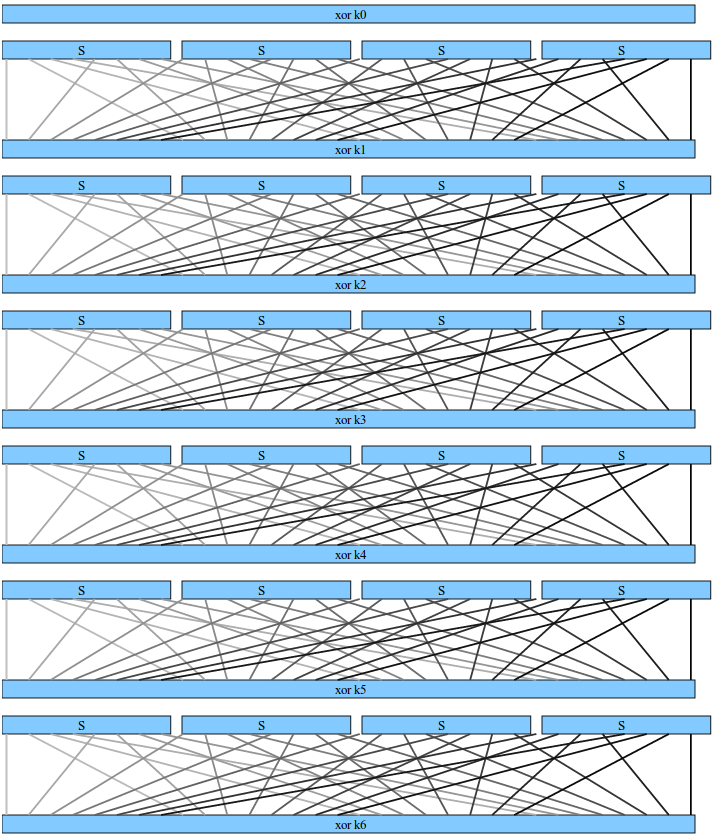
\includegraphics[width=\textwidth]{diagrams/bit}
\caption[Visualisation of UnsubA Permutation emphasising Bit Location]{A visualisation of UnsubA showing how the bits get distributed under
the permutation layer.}
\label{fig:bit}
\end{figure}

\begin{figure}[P]
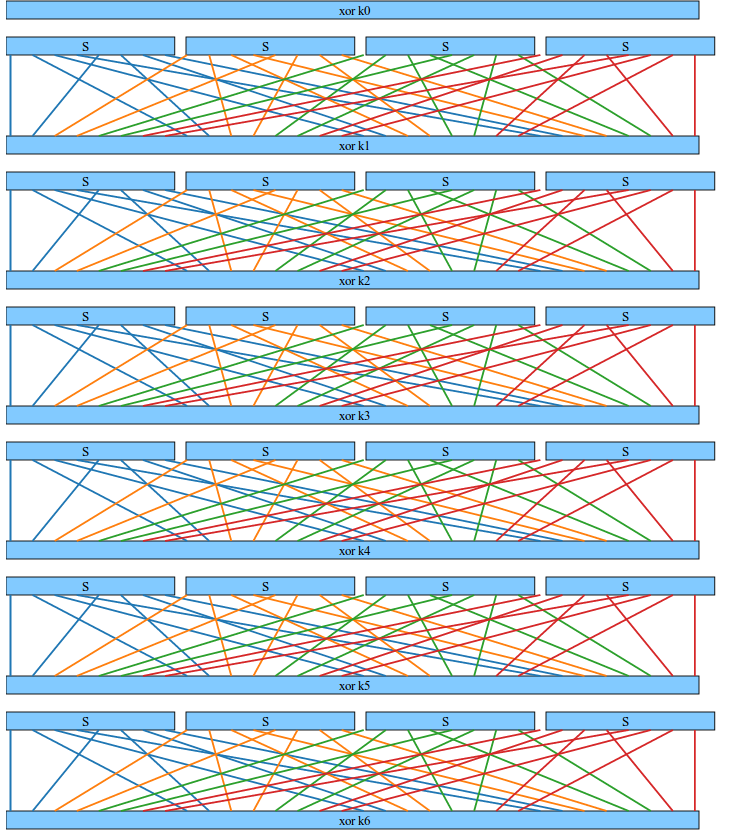
\includegraphics[width=\textwidth]{diagrams/sbox}
\caption[Visualisation of UnsubA Permutation emphasising Sbox Origin]{A
visualisation of UnsubA illustrating where the outputs of each sbox is
distributed by the permutation layer. Each different colour indicates a
different sbox origin, the lines indicate where each bit of the output of the
sbox is permuted to.}
\label{fig:sbox}
\end{figure}

\begin{figure}[P]
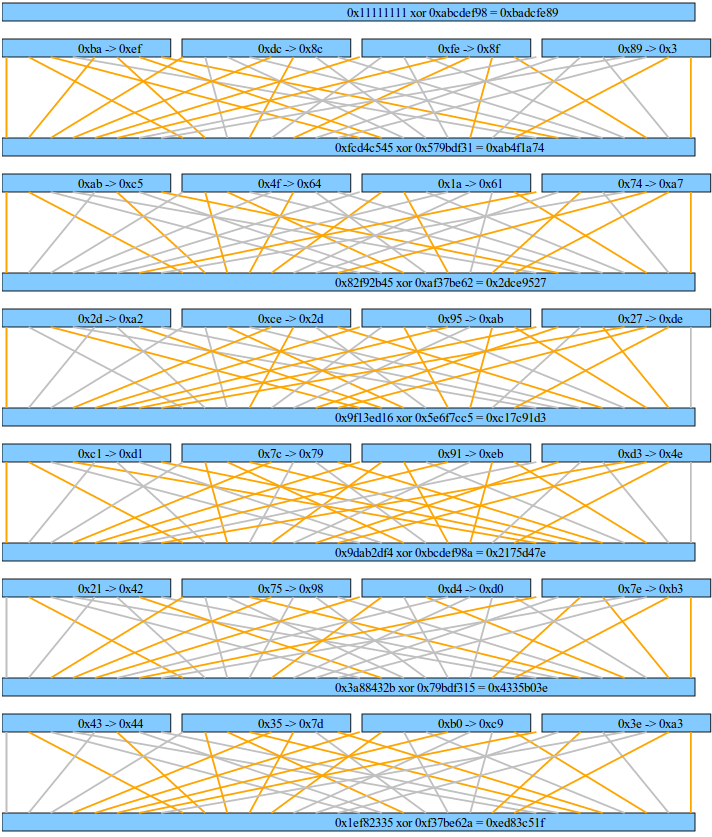
\includegraphics[width=\textwidth]{diagrams/encryption}
\caption[Visualisation of UnsubA Encryption]{A visualisation of UnsubA detailing the encryption of \hex{11111111}
under the key \hex{abcdef98}. The long horizontal boxes indicate the key addition
stages, the boxes below them indicate the values given to the sboxes and the
values they output. The coloured lines give the non-zero bits given to the
permutation layer and where they get distributed to.}
\label{fig:enc}
\end{figure}
%*********************************************************************************************************
% REFERENCES
%*********************************************************************************************************
\newpage
\bibliography{diff_crypto}{}
\bibliographystyle{plain}

\end{document}
